\documentclass[12pt,oneside,a4paper]{book}

\usepackage[usenames,dvipsnames]{xcolor}


%% === nezbytné balíčky:
\usepackage{lmodern}
% \usepackage[T1]{fontenc}    % kódování písma
%\usepackage[IL2]{fontenc}  % kódování písma

\usepackage[utf8]{inputenc}     % vstupní znaková sada tohoto dokumentu: UTF-8
%\usepackage[cp1250]{inputenc}  % vstupní znaková sada tohoto dokumentu: Windows 1250
%\usepackage[latin2]{inputenc}  % vstupní znaková sada tohoto dokumentu: ISO Latin 2

\usepackage[czech, english]{babel} % česky psaná práce, typografická pravidla. Překládejte pomocí "latex.exe" nebo "pdflatex.exe"
%\usepackage{czech} % česky psaná práce. Překládejte pomocí "pdfCSlatex.exe" ("cslatex.exe" asi bude mít problém s balíkem geometry)

\usepackage[a4paper, hmarginratio=3:2]{geometry} % využití A4 stránky a nastavení okrajů (u vazby bude širší)

\usepackage{pdfpages} % pokud nemáte formulář "Zadání bak./dipl. práce" naskenovaný jako PDF, tak ZAKOMENTUJTE
\usepackage[hidelinks]{hyperref} % v PDF budou klikací odkazy ("hidelinks" je nebude rámovat)

%% === balíčky, které se mohou hodit:
%\usepackage{encxvlna} % postará se o spojky a předložky, které dle českých pravidel nesmí být na konci řádku. Dokumentace: http://texdoc.net/texmf-dist/doc/generic/encxvlna/encxvlna.pdf (chová se správně k "vnitřku" listings?)

\usepackage{graphicx} % balíček pro vkládání rastrových grafických souborů (PNG apod.)
%\usepackage{epsfig} % balíčky pro vkládání grafických souborů typu EPS
% \usepackage{float} % rozšířené možnosti umístění obrázků
% \restylefloat{table}
\usepackage{pifont}

%\usepackage{caption} % pro popisky obrázků, tabulek atd.

\usepackage{tabularx} % rozšířené možnosti tabulek
\usepackage{longtable}

\usepackage{tabu} % jiný balík pro rozšířené možnosti tabulek

\usepackage{listings}
 % balíček vhodný pro ukázky zdrojového kódu v~textu práce/příloh. Nutno nastavit! http://ftp.cvut.cz/tex-archive/macros/latex/contrib/listings/listings.pdf

% \usepackage[autoload=true]{jlcode}
\usepackage{amsmath} % balíček pro pokročilou matematickou sazbu
\usepackage{amsfonts}
% \usepackage{color} % pro možnost barevného textu
%\usepackage{fancybox} % umožňuje pokročilé rámečkování
\usepackage{url}
\usepackage{bm}
\usepackage{hyperref}
\usepackage{threeparttable}
\newtheorem{definition}{Definition}
\usepackage{subcaption}

%\usepackage{index} % nutno použít v případě tvorby rejstříku balíčkem makeindex
%\newindex{default}{idx}{ind}{Rejstřík} % zavádí rejstřík v případě použití balíku index
% \usepackage{csquotes}
% \MakeOuterQuote{"}

% \frenchspacing % za větou bude mezislovní mezera (v anglických textech je mezera za větou delší)
\widowpenalty=1000 % "síla" zákazu vdov (= jeden řádek ze začátku odstavce na konci stránky)
\clubpenalty=1000 % "síla" zákazu sirotků (= jeden řádek/slovo z konce odstavce samostatně na začátku stránky)
\brokenpenalty=1000 % "síla" zákazu zlomu stránky za řádkem, který má na konci rozdělené slovo

\topmargin=-15mm      % horní okraj trochu menší
\textwidth=150mm      % šířka textu na stránce
\textheight=240mm     % "výška" textu na stránce


\pagenumbering{arabic} % číslování stránek arabskými číslicemi
\pagestyle{plain}      % stránky číslované dole uprostřed


% \setlength\parskip{0.1pt}
% \parindent=20pt % odsazení 1. řádku odstavce
% \parskip=0pt   % mezera mezi odstavci

%% --- zde jsou zavedeny některé "konstanty" - některé musíte změnit! --- %%
\newcommand{\cvut}{České vysoké učení technické v~Praze}
\newcommand{\fjfi}{Fakulta jaderná a fyzikálně inženýrská}
\newcommand{\ksi}{Katedra softwarového inženýrství}
\newcommand{\km}{Katedra matematiky}
% \newcommand{\program}{Aplikace přírodních věd} % změňte, pokud máte jiný stud. program
\newcommand{\obor}{Aplikace informatiky v přírodních vědách} % změňte, pokud máte kurzívujiný obor

\newcommand{\druh}{Výzkumný úkol} % nebo "Diplomová práce"
\newcommand{\woman}{a} % pokud jste ŽENA, ZMĚŇTE na: ...{\woman}{a} (je to do Prohlášení)

\newcommand{\logoCVUT}{
\includegraphics{symbol_cvut_konturova_verze_cb.pdf}} % logo ČVUT -- podle grafického manuálu ČVUT platného od prosince 2016. Pokud nevyhovuje PDF-verze, tak použijte jinou variantu loga: https://www.cvut.cz/logo-a-graficky-manual -> "Symbol a logo ČVUT v Praze"). Pokud chcete logo úplně vynechat, zadejte místo "\includegraphics{...}" text "\vspace{35mm}"

% přesně podle formuláře "Zadání bak./dipl. práce" VYPLŇTE:
\newcommand{\nazevczT}{Optické rozpoznávání znaků \\ na naskenovaných historických plakátech pomocí \\nejmodernějších metod}    % český název práce (přesně podle zadání!)
\newcommand{\nazevenT}{Optical Character Recognition \\on Scanned Historical Posters Using the State-of-the-Art Methods}          % anglický název práce (přesně podle zadání!)
\newcommand{\nazevcz}{Optické rozpoznávání znaků na naskenovaných \\historických plakátech pomocí nejmodernějších metod}    % český název práce (přesně podle zadání!)
\newcommand{\nazeven}{Optical Character Recognition on Scanned Historical Posters Using the State-of-the-Art Methods}          % anglický název práce (přesně podle zadání!)
\newcommand{\autor}{Anna Gruberová}   % vyplňte své jméno a příjmení (s akademickým titulem, máte-li jej)
\newcommand{\vedouci}{Ing. Adam Novozámský, Ph.D.} % vyplňte jméno a příjmení vedoucího práce, včetně titulů, např.: Doc. Ing. Ivo Malý, Ph.D.
\newcommand{\pracovisteVed}{Computer Vision Lab, Institute of Visual Computing \& Human-Centered Technology, TU Wien - Faculty of Informatics} % ZMĚŇTE, pokud vedoucí Vaší práce není z KSI
\newcommand{\konzultant}{--} % POKUD MÁTE určeného konzultanta, NAPIŠTE jeho jméno a příjmení
\newcommand{\pracovisteKonz}{--} % POKUD MÁTE konzultanta, NAPIŠTE jeho pracoviště

% podle skutečnosti VYPLŇTE:
\newcommand{\rok}{2022}  % rok odevzdání práce (jen rok odevzdání, nikoli celý akademický rok!)
\newcommand{\kde}{Praze} % studenti z Děčína ZMĚNÍ na: "Děčíně" (doplní se k "prohlášení")

\newcommand{\klicova}{Optické rozpoznávání znaků, rozpoznávání textu, automatizace}   % zde NAPIŠTE česky max. 5 klíčových slov
\newcommand{\keyword}{Optical Character Recognition, Text Recognition, Automation}       % zde NAPIŠTE anglicky max. 5 klíčových slov (přeložte z češtiny)
\newcommand{\abstrCZ}{Optické rozpoznávání znaků z obrazových dat je žádanou úlohou v dnešním světě, jelikož pro člověka je již nemožné bez automatizace zpracovat velké množství obrazových dat. Vídeňská knihovna vlastní nad 350 tisíc digitalizovaných historických plakátů, z nichž je třeba extrahovat zobrazený text. Cílem této práce je zmapovat vybrané existující metody rozpoznávání textu a porovnat je na základě testů na vybraných datasetech.}


% zde NAPIŠTE abstrakt v češtině (cca 7 vět, min. 80 slov)
\newcommand{\abstrEN}{Optical character recognition from image data is a demanding task in today's world, because it is already impossible for humans to process a large amount of image data without automation. The Vienna Library owns over 350,000 digitized historical posters, from which the displayed text must be extracted. The aim of this work is to map selected existing text recognition methods and compare them based on tests on selected datasets.} % zde NAPIŠTE abstrakt v angličtině

\newcommand{\prohlaseni}{Prohlašuji, že jsem svou bakalářskou práci vypracoval\woman{} samostatně a použil\woman{} jsem pouze podklady (literaturu, projekty, SW atd.) uvedené v přiloženém seznamu.} % text prohlášení můžete mírně upravit :-)

\newcommand{\podekovani}{.} % NAPIŠTE poděkování, např. svému vedoucímu:
% Děkuji Ing. Eleonoře Krtečkové, Ph.D. za vedení mé bakalářské práce a za podnětné návrhy, které ji obohatily.
% NEBO:
% Děkuji vedoucímu práce doc. Pafnutijovi Snědldítětikaši, Ph.D. za neocenitelné rady a pomoc při tvorbě bakalářské práce.

\newcommand{\ti}{\textit} % zkrácený příkaz pro kurzívu
\newcommand{\tb}{\textbf} % zkrácený příkaz pro tučné písmo
\newcommand{\tn}{\texttt} % zkrácený příkaz pro neproporcionalni písmo

% Vzhled kodu - lstlistings - python
\definecolor{codegreen}{rgb}{0,0.6,0}
\definecolor{codegray}{rgb}{0.5,0.5,0.5}
\definecolor{framegray}{rgb}{0.8,0.8,0.8}
\definecolor{codepurple}{rgb}{0.58,0,0.82}
\definecolor{backcolour}{rgb}{0.95,0.95,0.92}

\lstdefinestyle{mystyle}{
    language=Python,
    frame=single,
    rulecolor=\color{framegray},
    commentstyle=\color{codegreen},
    keywordstyle=\color{magenta}\bfseries,     numberstyle=\tiny\color{codegray},
    stringstyle=\color{codepurple},
    basicstyle=\ttfamily\footnotesize,
    breakatwhitespace=false,         
    breaklines=true,                 
    captionpos=t,                    
    keepspaces=true,                 
    numbers=left,                    
    numbersep=5pt,                  
    showspaces=false,                
    showstringspaces=false,
    showtabs=false,                  
    tabsize=2
}
\lstset{style=mystyle}

\renewcommand{\lstlistingname}{Function}

%-----------------------------------------------

\newenvironment{repl}
{\fontfamily{cmvtt}\selectfont \begin{mdframed}

}{\end{mdframed}}

\usepackage[linewidth=1pt]{mdframed}


\newcolumntype{L}{>{\centering\arraybackslash}m{2cm}}
\newcolumntype{N}{>{\centering\arraybackslash}m{1.7cm}}
\newcolumntype{M}{>{\centering\arraybackslash}m{1.6cm}}
\newcolumntype{K}{>{\centering\arraybackslash}m{1.5cm}}
\newcolumntype{S}{>{\centering\arraybackslash}m{1cm}}
\renewcommand{\arraystretch}{1.3}

\newcommand{\cmark}{\textcolor{green!80!black}{\ding{51}}}
\newcommand{\xmark}{\textcolor{red}{\ding{55}}}





% todo notes
\usepackage[colorinlistoftodos]{todonotes}

\begin{document}
%%%%%%%%%%%% TITULNÍ STRANA -- na následujících cca 30 řádků NESAHEJTE!!!  Generuje se AUTOMATICKY %%%%%%%%%%%%
\thispagestyle{empty}

\begin{center}
	{\LARGE
		\cvut\par
		\fjfi
	}
    \vspace{10mm}

    \begin{tabular}{c}
		\tb{\ksi} \\[3pt]
		\tb{Obor: \obor}\\
    \end{tabular}

   \vspace{10mm} \logoCVUT \vspace{15mm}

   {\huge \tb{\nazevczT}\par}
   \vspace{5mm}
   {\huge \tb{\nazevenT}\par}

   \vspace{15mm}
   {\Large \MakeUppercase{\druh}}

   \vfill
   {\large
    \begin{tabular}{ll}
    Vypracoval: & \autor\\
    Vedoucí práce: & \vedouci\\
    Rok: & \rok
    \end{tabular}
   }
\end{center}

\clearpage{\pagestyle{empty}\cleardoublepage} % prázdná stránka za tou "titulní", bez čísla

%%%%%%%%%%%% ZADÁNÍ PRÁCE %%%%%%%%%%%%
% Zadání (podepsané děkanem!) musíte NASKENOVAT. Ideálně jako 2stránkové PDF (soubor "zadani_cele.pdf").
% Před svázáním to v jednom výtisku VYMĚNÍTE ZA ORIGINÁLNÍ ZADÁNÍ (podepsané děkanem fakulty)!
\newpage  % SEM NESAHEJTE!
\thispagestyle{empty} % SEM NESAHEJTE!

%% zde podle toho, jak jste zadání naskenovali, VYBERTE variantu A, B nebo C:
%
% --- varianta A: zadání naskenované jako 2stránkové PDF:
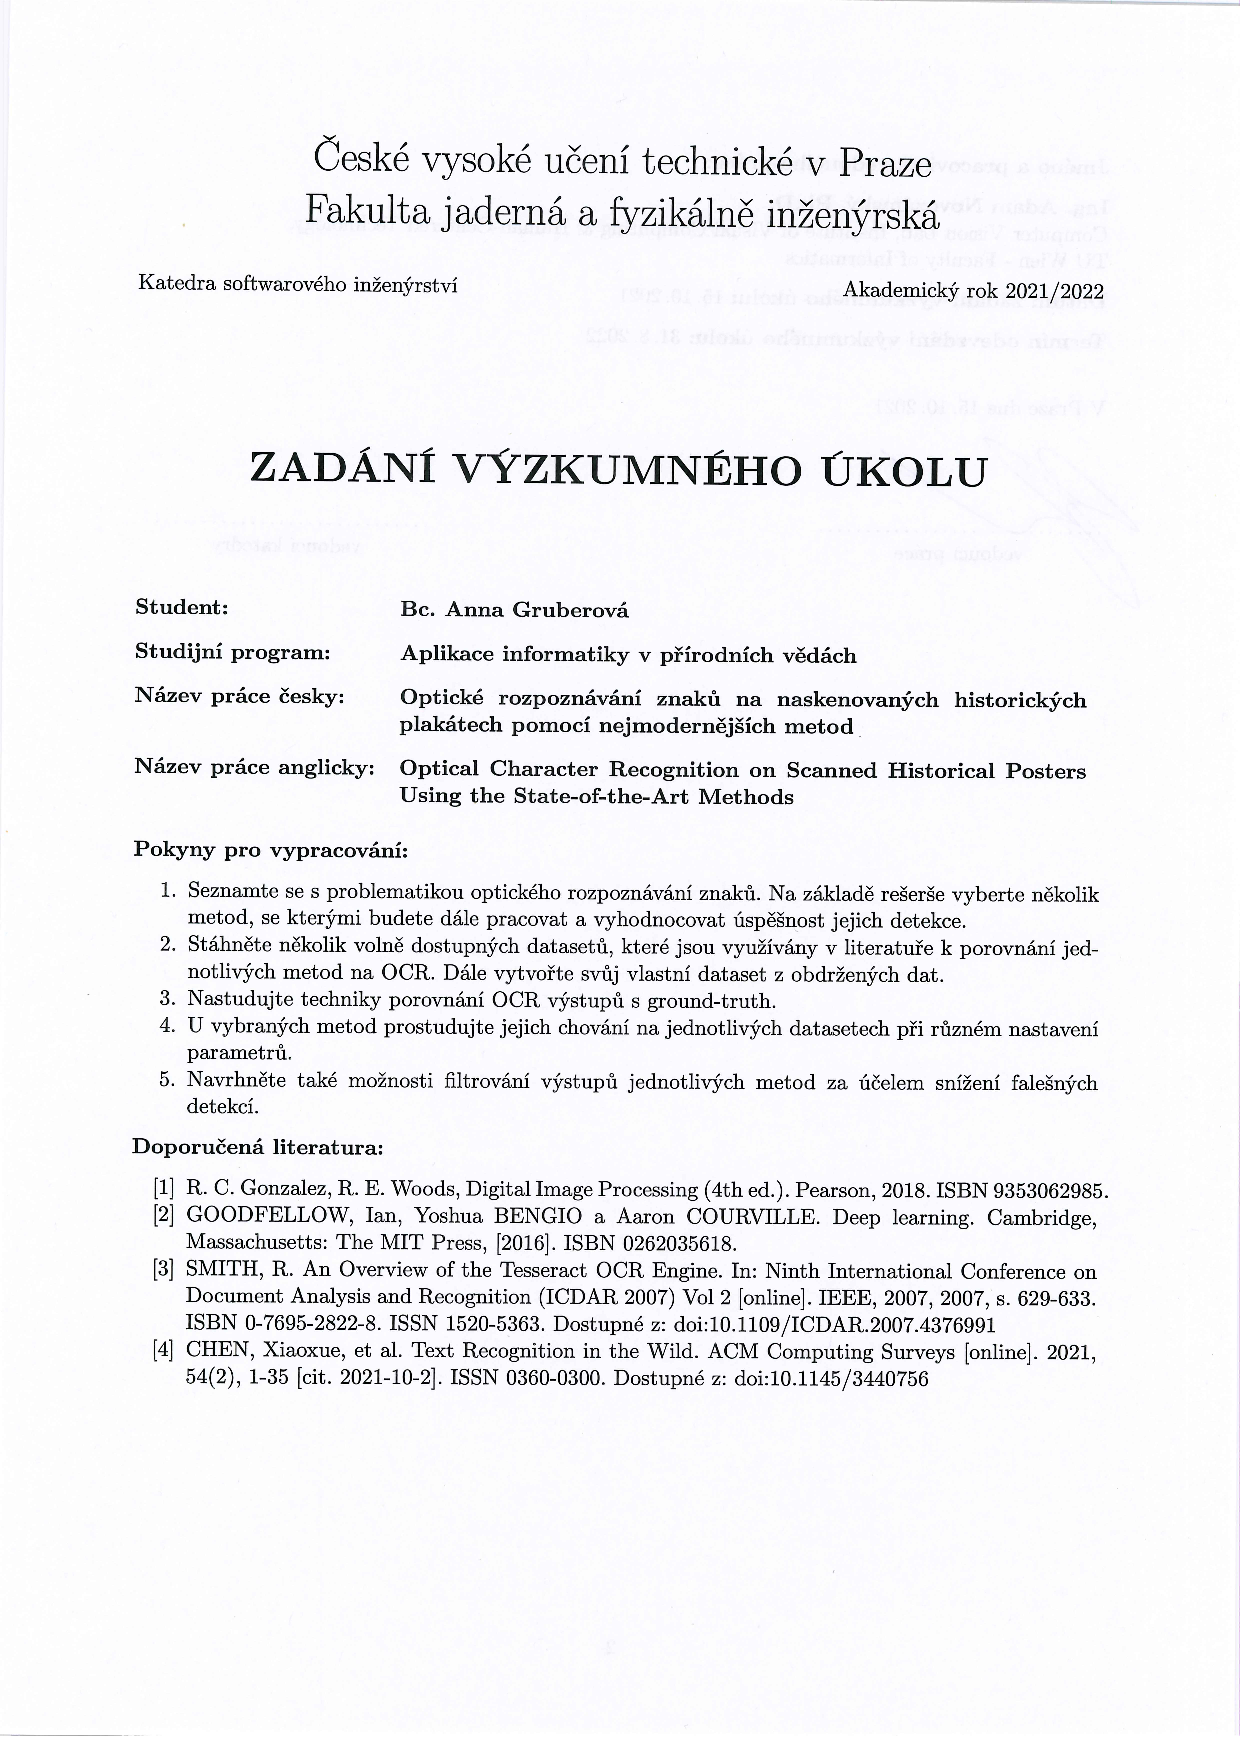
\includepdf[pages={1,2}]{zadani.pdf} % NAHRAĎTE správným souborem!!!!DOPLNIT
%
%% --- varianta B: zadání naskenované jako jednotlivé stránky:
%\includepdf[pages={1}]{zadani1.pdf} % 1. strana zadání v PDF
%\includepdf[pages={1}]{zadani2.pdf} % 2. strana zadání v PDF
%
%% --- varianta C: zadání naskenované jako 2 samostatné obrázky:
%% 1. strana zadání
%\begin{center}
%     \includegraphics[width=1\textwidth]{zadani1.jpg}
%\end{center}
%% 2. strana zadání
%\newpage  % SEM NESAHEJTE!
%\thispagestyle{empty} % SEM NESAHEJTE!
%\begin{center}
%     \includegraphics[width=1\textwidth]{zadani2.jpg}zada
%\end{center}


%%%%%%%%%%%% Prohlášení -- SEM NESAHEJTE! Generuje se automaticky z výše nastavených maker \kde{} a \prohlaseni{}. %%%%%%%%%%%%
\newpage % SEM NESAHEJTE!
\thispagestyle{empty}  % SEM NESAHEJTE!

~ % SEM NESAHEJTE!
\vfill % prázdné místo. SEM NESAHEJTE!

\tb{Prohlášení} % SEM NESAHEJTE!

\vspace{1em} % vertikální mezera. SEM NESAHEJTE!
\prohlaseni

\vspace{2em}  % SEM NESAHEJTE!
\hspace{-0.5em}\begin{tabularx}{\textwidth}{X c}  % SEM NESAHEJTE!
V \kde\ dne .................... &........................................ \\	% SEM NESAHEJTE!
	& \autor
\end{tabularx}	% SEM NESAHEJTE!


%%%%%%%%%%%% Poděkování  %%%%%%%%%%%%
\newpage
\thispagestyle{empty}

~
\vfill % prázdné místo


% -- následující kus kódu (do "%%%%%%%%%%%% ABSTRAKT") můžete odstranit, pokud nechcete psát poděkování:
\tb{Poděkování}

\vspace{1em} % vertikální mezera
\podekovani
\begin{flushright}
\autor
\end{flushright}  % <------- tady končí stránka s poděkováním


%%%%%%%%%%%% ABSTRAKT atp. Je generován AUTOMATICKY podle maker nastavených na začátku souboru) %%%%%%%%%%%%
\newpage   % SEM NESAHEJTE!
\thispagestyle{empty}   % SEM NESAHEJTE!

% příprava:    (na následujících 8 řádků NESAHEJTE!)
\newbox\odstavecbox
\newlength\vyskaodstavce
\newcommand\odstavec[2]{%
    \setbox\odstavecbox=\hbox{%
         \parbox[t]{#1}{#2\vrule width 0pt depth 4pt}}%
    \global\vyskaodstavce=\dp\odstavecbox
    \box\odstavecbox}
\newcommand{\delka}{115mm} % šířka textů ve 2. sloupci tabulky

% použití přípravy:    % dovnitř "tabular" vůbec NESAHEJTE!
\begin{tabular}{ll}
  {\em Název práce:} & \odstavec{\delka}{\bf \nazevcz} \\ [1em]
  % \multicolumn{2}{l}{\bf \nazevcz} \\[1em]
  {\em Autor:} & \autor \\[1em]
  % {\em Studijní program:} & \program \\
  {\em Obor:} & \obor \\
  {\em Druh práce:} & \druh \\[1em]
  {\em Vedoucí práce:} & \odstavec{\delka}{\vedouci\\ \pracovisteVed} \\
  {\em Konzultant:} & -- %\odstavec{\delka}{\konzultant \\ \pracovisteKonz}  % VYMAŽTE text "-- %" v případě, že jste neměli konzultanta
 \\[1em]
  \multicolumn{2}{l}{\odstavec{\textwidth}{{\em Abstrakt:} ~ \abstrCZ  }} \\[1em]
  {\em Klíčová slova:} & \odstavec{\delka}{\klicova} \\[2em]

  {\em Title:} & \odstavec{\delka}{\bf \nazeven} \\ [1em]
  {\em Author:} & \autor \\[1em]
  \multicolumn{2}{l}{\odstavec{\textwidth}{{\em Abstract:} ~ \abstrEN  }} \\[1em]
  {\em Key words:} & \odstavec{\delka}{\keyword}
\end{tabular}



%%%%%%%%%%%% Obsah práce ... je generován AUTOMATICKY %%%%%%%%%%%%
\newpage  % SEM NESAHEJTE!
\parskip=0pt
\tableofcontents % SEM NESAHEJTE!
\parskip=7pt
\newpage % SEM NESAHEJTE!


%--------------------------------------------------------
%|         Zde začíná SAMOTNÁ PRÁCE (text)              |
%--------------------------------------------------------

% \chapter*{Úvod} % SEM NESAHEJTE!
% \addcontentsline{toc}{chapter}{Úvod} % SEM NESAHEJTE!
%
%

\chapter*{Introduction}
\addcontentsline{toc}{chapter}{Introduction}


This paper is aimed at optical character recognition and focuses on comparison of different methods that are used in this branch of image processing. The goal of the paper is to test selected methods with various parameters on different datasets. One of the datasets includes historical posters from Vienna City Library. This dataset needed to be selected from a broad database of posters and manually labeled.

In the first chapter I introduced terms used in optical image recognition and described main tasks -- text detection and recognition. This is followed by a brief description of the structure of text image data accompanied by commonly used dataset examples.

The next chapter is dedicated to neural networks, which play a leading role in image recognition and in reading text tasks. I proceed from the basic network architecture to more complex networks that were developed for image and text recognition.

In the third chapter is a description of four selected methods I had chosen as methods to be tested for the purpose of this paper.

The last chapter is about performed experiments. It includes information of selected datasets, a description of implemented functions and above all a discussion about results obtained in the experiments.
\chapter{Optical Character Recognition}

Optical character recognition (OCR) is a branch of digital image processing. Its aim is to detect and convert a text on an image into a machine-readable text. This discipline can be divided into three similar, yet different tasks: reading text on scanned printed documents, reading of handwritten texts and scene text recognition (also called text in the wild). The first task is very well developed, first successful results date back to the second half twentieth and were used in commercial sector \cite{ocrhist}. If we assume the handwritten text is on scanned single colored paper or created using a digital pen and that it was written legibly and without omitting letters in words due to fast writing, then recognition is similar to printed documents. The last task -- scene text recognition (STR) is the most challenging one. 
The main factors that make STR a more difficult task are listed below.\cite{chen2021text, raisi2020text}

\begin{itemize}
    \item Complex background: in scanned documents background is white and without  a distinctive pattern (omitting lines is an easy preprocessing task), while in scene images there are objects that can be mistaken for letters.
    \item Text diversity: text can appear in various colors, fonts, sizes or orientations.
    \item Distortions: photographs often suffer from noise due to bad illumination, also from motion or out-of-focus blurring, perspective distortion due to the capturing angle. Other problems come from the insufficient resolution that might be set on the camera.
\end{itemize}

Apart from these main categories of image text data there exist born-digital images (e. g. web advertisements or any cases where text was digitally added on images or videos) and poster/newspaper images. These share with scene images the diversity of text but are free from visual distortions caused by cameras. Examples of different image data are in the chapter \ref*{ch:datasets}. 

Digital reading of a text on an image consists of two main tasks -- text detection and text recognition. Both processes are described in the next sections.

\section{Text Detection}

The first phase of digital text processing is to detect the text regions on the image. The goal is to determine a bounding box surrounding a group of letters -- usually one word, but it can be also a text line consisting of few words. This box may be a bounding rectangle or a polygon which is more accurate for curved or skewed text. It is ideal when the bounding box contains the letters with as little background as possible. % When text candidates are found they have to be verified.
Methods used for text detection can be categorizes into formerly used classical machine learning methods and deep learning methods. 

\subsection*{Classical Methods}

Classical methods include connected component methods and sliding window methods. In the latter method an image is scanned with a moving window of certain size. In each position of the window features are computed, for example, standard deviation or histogram of oriented gradients and are compared with values known from training images with text.    This approach does not have a good response for scene images, because many objects can be misunderstood as letters and vice versa. Connected component based methods extract from the image features like color, texture, edges or corners. Then they are classified either as text or non-text by a traditional classifier such as support vector machines, nearest neighbor or random forest. Detected letters are then combine into words or text lines if desired \cite{raisi2020text}. Classical methods are generally not very successful with scene images where most of the observed values are negatively influenced by distorting factors listed above. In recent years the development of neural networks enabled a new, efficient way of detecting text in images.

\subsection*{Deep Learning Methods}

Deep learning methods are faster, more precise than the classical methods. They are automated and need less of human assistance therefore they can process bigger amounts of data. Another advantage is that algorithms can be generalized and used for other image detection tasks. Most of the state-of-the-art methods utilize convolutional neural network (CNN). Deep learning methods can be split into bounding-box regression based, segmentation based and hybrid methods according to the survey of Raisi et al. \cite{raisi2020text}.

Bounding-box regression based methods treat text as an object and predict directly the bounding box around text. However, the bounding boxes have different aspect ratio than typical objects, because text is usually long and thin. Some methods decompose the text on smaller units and concentrate on distances between the units. These methods are hard to tune during training an usually fail on distinctly curved text. Examples of bounding-box methods are TextBoxes \cite{liao2017textboxes}, TextBoxes++ \cite{liao2018textboxes++} or EAST \cite{zhou2017east}. Segmentation based methods investigate the image at pixel level. The image data are processed by a CNN which produces a segmentation map from which a bounding box is generated. An example of this method is PSENet \cite{wang2019shape}. Hybrid methods combine the features obtained by regression and the segmentation map from CNN. The segmentation methods tend to return false positive detection. They select pixels that are not text at the borders of letters or when there is a complicated background. Hybrid methods further process the results from segmentation and precisely detect text. Example methods are PMTD \cite{liu2019pyramid}.

A popular method in recent years is Character Region Awareness for Text Detection -- CRAFT. This method in contrast to the previously mentioned methods detects text based on character level rather than word (group of characters) level. CRAFT trains a CNN which produces two results for a character -- a region score and an affinity score. "The region score represents the probability that the given pixel is the center of the character and the affinity score represents the center probability of the space between adjacent characters" \cite[page 3]{craft2}. Because this method goes over individual characters it performs very well on curved and deformed text and outperforms 15 popular detection methods according to the authors of CRAFT in their paper \cite{craft2}.

\section{Text Recognition}

\chapter{Neural Networks}

% Pridat uvodni povidani k sitim, proc, a co se deje v nasledujici kapitole
% ---------------------------------------------------------------------------

% Perceptron

A perceptron unit is able to find a linear boundary between two separable classes. In \emph{n}-dimensional space we talk about a separating hyperplane. The following equation \begin{equation} \bm{w}^\top \bm{x}+ w_{n+1} = 0\end{equation} is a vector form of the hyperplane equation, where $\bm{w}$ is a weight, \emph{n}-dimensional column vector, $\bm{x}$ is also \emph{n}-dimensional vector and it contains the coordinates of a point, which is being classified, $w_{n+1}$ is a bias. We can simplify the notation by creating a \emph{n+1}-dimensional vectors: $\bm{x} = [x_1, \dots, x_n, 1]^\top$ and $\bm{w} = [w_1, \dots, w_n, w_{n+1}]^\top$.
We want to find a weight coefficients that satisfies the following property:
\begin{equation}
\bm{w}^\top \bm{x} > 0 \qquad \bm{x} \in {class_1}\end{equation}
\begin{equation}
\bm{w}^\top \bm{x} < 0 \qquad \bm{x} \in {class_2}
\end{equation}
Then the perceptron learning algortihm can be described as follows:

For any $\bm{x}(k)$, at step $k$:
\begin{enumerate}
    \item If $\bm{x}( k ) \in class_1$ and $\bm{w}^\top \bm{x} \leq 0$ , let    
    \begin{equation}\bm{w} ( k + 1 ) = \bm{w} ( k ) + \alpha  \bm{x }( k )\end{equation}
    \item If $\bm{x}( k ) \in class_2$ and $\bm{w}^\top \bm{x} \geq 0$ , let   
    \begin{equation}\bm{w} ( k + 1 ) = \bm{w} ( k ) - \alpha  \bm{x }( k )\end{equation}
    \item Otherwise, let 
    \begin{equation}\bm{w} ( k + 1 ) = \bm{w} ( k )\end{equation}
\end{enumerate}

where $\bm{w}(1)$ is arbitrary and $\alpha > 0$ is a constant called learning rate. Sum of the products, $\sum_{k=1}^{n}w_kx  + w_{n+1}$ is then passed through an activation function. In case of perceptron it is a threshold function returning either 1, when $\bm{x}$ belongs to $class_1$, or -1 when it belongs to the second class $class_2$. In Figure \ref*{img:percneuron}.a.
is shown a model of a perceptron.\cite{raisi2020text}

% obrazky perceptronu a neuronu vedel sebe, l jsou vrstvy
\begin{figure}[hbtp]
    \centering
    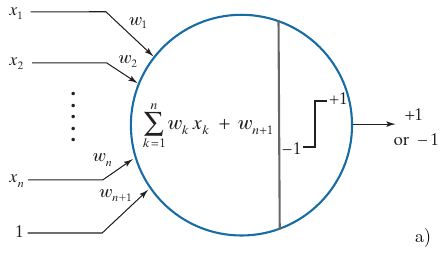
\includegraphics[scale=0.41]{obrazky/perceptron.png}
    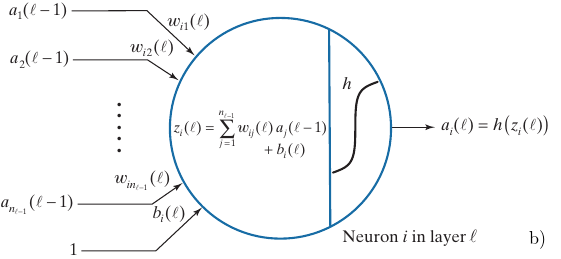
\includegraphics[scale=0.41]{obrazky/artneuron.png}

    \caption{Model of a perceptron unit (a), model of an artificial neuron (b) with used operations. The letter $h$ denotes an activation function, $l$ denotes a particular layer in a multilayer network. The element on the right is sometimes called a sigmoid neuron.\cite{DIP}}
    \label{img:percneuron}
\end{figure}

Linearly separable data are rather rare in real life problems. One possibilities is to use more perceptron units, however, the solution comes with neural networks and computing elements called artificial neurons. These elements are similar to perceptrons as they perform the same computations, but have a different attitude to processing the results. Schematics of a perceptron unit and an artificial neuron can be comapred in figure \ref*{img:percneuron}.
The perceptron activation function is very insensitive to small signals which can lead to false results. If the activation function is changed from a hard threshold to smooth function, results are then handled more carefully. There are few commonly used smooth activation functions, such as sigmoid, hyperbolic tangent or ReLu (rectifier linear unit) function. In Figure %obrazek
are the equations and shapes of the mentioned functions.\cite{DIP}

% obrazky funkci. h je jakoznaceni aktivacni funkce
 
A generic neural network is depicted in Figure \ref*{img:fullyNN}.  By layer we understand a group of neurons, usually symbolized in a column. First layer contains the input vector $\bm{x}$, then every other layer contains the activation values of neurons in this layer. The conntecting lines between each two neurons signifies a fully connected neural network, where  output of every neuron from one layer is used as input for neurons in the following layer. Values of initial layer are known and also are the last output values, all neurons (and layers) between first and last layer are therefore called hidden. When there are more then one hidden layer we talk about deep neural network. Usually the number of output neurons is equal to the number of observed classes. For the rest of this chapter we will assume that there are no loops in the network.\cite{DIP}

\begin{figure}[hbtp]
    \centering
    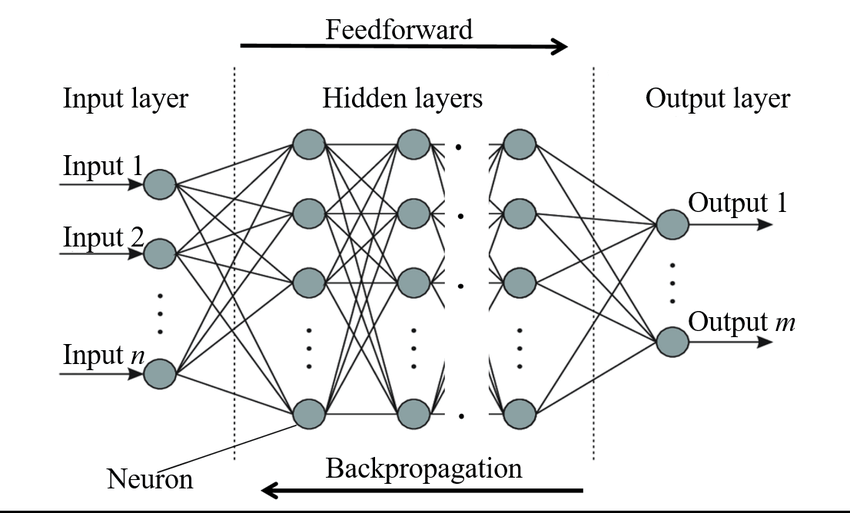
\includegraphics[scale=0.5]{obrazky/fullyNN.png}

    \caption{Fully connected neural network with processes.\cite{nn1}}
    \label{img:fullyNN}
\end{figure}

A forward pass through neural network maps the values of vector $\bm{x}$ (the input layer)  to the output layer, thus to determine the class of the vector $\bm{x}$. Steps of a forward pass can be written in matrix notation. This aproach is good for computing simultaneously with multiple input vectors and all neurons in one layer. The forward pass can be described in three steps:

\begin{enumerate}
    \item Input \begin{equation}\bm{A}(1)=\bm{X}\end{equation}
    \item Feedforward step 
    \begin{equation}\mbox{For } l = 2, \dots, L \qquad \bm{Z}(l) = \bm{W}(l)\bm{A}(l-1)+\bm{B}(l) \mbox{, } \bm{A}(l)=h(\bm{Z}(l))\end{equation}
    \item Output \begin{equation}\bm{A}(L)=h(\bm{Z}(L))\end{equation}
\end{enumerate}

Matrix $\bm{W}(l)$ contains all weight vectors of all nodes in one layer $l$, $\bm{X}$ contains input vectors, $\bm{A}(l)$ contains output values from layer $l$, $\bm{B}$ is the matrix of biases, $\bm{Z}(l)$ contains the net inputs to neurons in layer $l$, $h$ is an activation function. This process of predicting works when we know the right values of weights and biases. These can be obtained by training a neural network via backpropagation.\cite{DIP}

During training of neural network we work with data where it is known for each sample to which class it belongs. This means that we know the values of all otuput neurons in the net. However, we do not know the values of outputs of hidden neurons. A process called backpropagation is used to obtain information about hidden neurons. It can be devided into four steps. These steps are repeated until the value of cost function is reduced to a desired level. One repetition is called an epoch, thus the number of iterations is the number of epochs used for training the network. \cite{DIP}

\begin{enumerate}
    \item Input of data from training set.
    \begin{equation}\bm{A}(1)=\bm{X}\end{equation}
    \item A forward pass to classify the data into class and determine the error of misidentified classes (sometimes this error function is called cost function) based on ground thruth from the training data.
    \begin{align}
        \begin{split}
            \mbox{For } l = 2, \dots, L \qquad & \bm{Z}(l) = \bm{W}(l)\bm{A}(l-1)+\bm{B}(l) \mbox{, }  \\
            & \bm{A}(l)=h(\bm{Z}(l)) \mbox{, }  \\
            & \bm{D}(L)=(\bm{A}(L)-\bm{R}) \odot h'(\bm{Z}(L))
        \end{split}
    \end{align}

    \item A backward pass that sends the output error back through the network, where changes to update neuron paramters are computed.
    \begin{equation}
        \mbox{For } l = L - 1 , L - 2 , \dots , 2 \qquad \bm{D}(l) = ( \bm{W}^\top ( l + 1 ) \bm{D} (l + 1 ) \odot h' ( \bm{Z} (l) )
    \end{equation}
    \item An update of weights and biases of neurons.
    \begin{align}
        \begin{split}
            \mbox{For } l = 2, \dots, L \qquad & \bm{W}(l) = \bm{W}(l) - \alpha \bm{D}(l)\bm{A}^top(l-1) \mbox{, }  \\
            & \bm{b}(l)= \bm{b}(l) - \alpha  \sum_{k=1} ^{n_p}  {\delta}_k(l) \mbox{, }   \\
            & \bm{D}(L)=(\bm{A}(L)-\bm{R}) \odot h'(\bm{Z}(L)) \mbox{, }  \\
            & \bm{B}(l) \mbox{ consist of horizontally stacked vectors } \bm{b}(l) \\ 
            & \mbox{for } n_p \mbox{ times,} \\
            & \bm{\delta}_k(l) \mbox{ are the columns of matrix } \bm{D}(l) \mbox{,}
        \end{split}
    \end{align}
\end{enumerate}
where $\bm{W}(l)$ is the matrix of weights of all nodes in one layer $l$ for the inputs from $\bm{X}$, which contains multiple input vectors, $\bm{A}(l)$ contains output activation values from layer $l$, $\bm{B}$ are the biases, $\bm{Z}(l)$ contains the net inputs to neurons in layer $l$, $\bm{\delta}(l)$ tells us the rate of error change with respect to a change in the net input to any neuron in the network $\delta_k(l) = $, $\alpha$ is the  learning rate used in training, $h$ is an activation function.  
$\bm{W}(1)$ and  $\bm{B}(1)$ are set as random small numbers when initializing the process.\cite{DIP}

The error function for all output neurons for a single input $\bm{x}$ is defined as
\begin{equation} E = \sum_{j=1} ^{n_L} E_j = \frac{1}{2}\sum_{j=1} ^{n_L} (r_j-a_j(L)) = \frac{1}{2} ||\bm{r} - \bm{a}(L)||^2 \end{equation}

where $\bm{r}$ is a desired response for a given input $\bm{x}$, $\bm{a}(L)$ is the output of last layer in the network, in the last term is used the notation of the Euclidan vector norm. The error for all input vectors\footnote{a total  network output error} is equal to the sum of the individual errors. \cite{DIP}

\section{Convolutional Neural Networks}

The procedures described in the previous part dealt only with the case where the input data are in the form of a vector. In optical character recognition we work with image data that are not primarily represented as vector but as a matrix of pixel values. The matrix can be linearized from 2D to 1D when indeces are mapped gradually. However,  this approach does not consider spatial relationships that may be present among specific pixels. For examples edge or color similarities which are significant in text detection. Convolutional neural network (CNN) accepts 2D matrix as input and extracts features from the given image, these features are then fed to a classic fully connected neural network. A diagram describing  a simple CNN is in Figure \ref*{img:CNN}. We will discuss individual steps visible in this figure below.\cite{DIP}

\begin{figure}[hbtp]
    \centering
    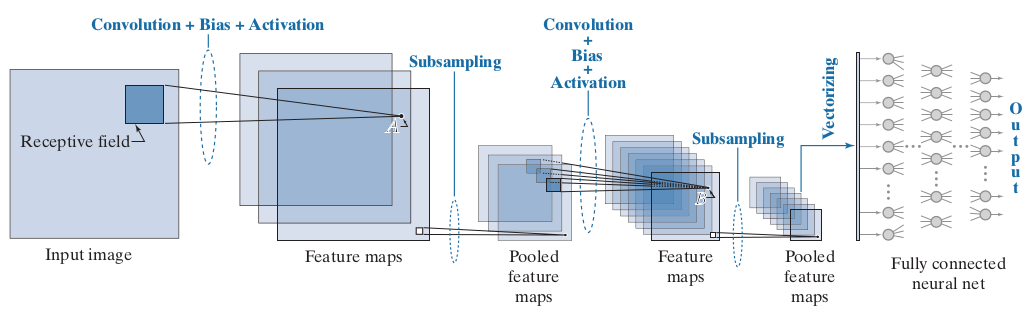
\includegraphics[scale=0.4]{obrazky/CNN.png}

    \caption{A simple CNN with LeNet architecture.\cite[altered]{DIP}}
    \label{img:CNN}
\end{figure}

First, a region of of pixels of the input image, a receptive field,  is selected. This field is moved over the image with a certain step. At each position a convolution is performed and values are stored in a 2D matrix. The size of the step determines the size of the resulting matrix (for example step of size two reduces the resolution of the image by one half). To each value obtained by convolution a bias is added and then is passed through an activation function. The new matrix thus obtained is called feature map. A single feature map is generated with same weights in convolution kernel and same bias, because this way a same feature is detected through the image. For another feature map different weight and bias is used. A group of feature maps in a CNN are called a convolutional layer. After the convolution step pooling is performed (sometimes called subsampling).\cite{DIP}

\begin{definition}
    Let $f(x,y)$ be in image and $w$ a kernel of size $m \times n$. Convolution with kernel $w$ is denoted as 
    $(w\star f)$     and defined as
    \begin{equation}
        (w\star f)(x,y) = \sum_{u=-k} ^{k} \sum_{v=-l} ^{l} w(u,v) f(x-u, y-v).
    \end{equation}
\end{definition}

Pooling is responsible for reduction of output dimension and causes a translational invariance. It is done by dividing a feature map into $2 \times 2 $ adjacent (non-overlapping) regions, the four values in this region are replaced by only one value. Common pooling methods are: average pooling, the values in region are replaced by the average of the values; max pooling, the values are replaced by the maximal value from the region; $L_2$ pooling, the final value is obtained by computing the Euclidan norm of the four values. We obtain one matrix for each feature map from the convolution step. The bunch of matrices from the pooling step is called a pooling layer. The result of the last pooling layer is vectorized and sent to the fully connected neural network. The training procedure of the CNN is analogical to the training of a fully connected neural network. However, convolution is used instead of matrix multiplication and the output from fully connected network has to be converted into 2D matrix.\cite{DIP}

% napsat definici konvoluce Convolution!!!













\section*{Outline}

\begin{itemize}
    \item What is OCR 
    \item Datasets (types(synthetic, photos, scaned documents),problems(languages, noise, nonhorizontal text))
    \item Text detection
    \begin{itemize}
        \item Description
        \item Methods (CRAFT)
    \end{itemize}
    \item Text recognition
    \begin{itemize}
        \item Description
        \item Methods 
    \end{itemize}
    \item End-to-end systems (Annotating tool)
    \begin{itemize}
        \item[] Reading scanned documents
        \item EasyOCR
        \item keras-ocr
        \item Tesseract (PyTesseract)
        \item (Google Cloud Vision free) paid
        \item (AWS Recognition) paid 
        \item (Kili) paid
    \end{itemize}
    \item Results evaluation
    \begin{itemize}
        \item Comparison of output and ground-truth
        \item Bag of words
    \end{itemize}
    \item Testing methods on free datasets
    \item[] Description of datasets
    \item Using methods on historical posters    
    \item[] Description of dataset

\end{itemize}
\newpage

\chapter{Software}

\section{Scene text detection}

\section*{Methods}
\subsection{CRAFT}

Character Region Awareness for Text Detection (CRAFT) is framework for scene text detection. It uses a Convolutional Neural Network. It performs good also on curved or differently deformed texts. Its methodology is to localize individual characters then characters belonging to the same word (based on distance) can be connected into word box or polygon. After that bounding box is created around it and output contains the rectangle coordinates.\cite{craft2}

\section{Scene text recognition}

\section*{Methods}
\subsection{CRNN}

Convolutional Recurrent Neural Network

\section{End-to-end systems}

End-to-end system when given an image with text it can both detect and recognize the text and produces a string output of the text. The supply of such is wide, ranging from open source libraries for various programming languages to commercial softwares with modern GUI. New methods are still being developed as there is always space for improvement. New methods can come from commercial background or are developed for international OCR competitions. In the next section some of the free available tools are described.

\subsection{Tesseract}

Tesseract is an open source text recognition engine. It supports over 160 languages. Originally Tesseract was created by Hewlett-Packard in late 1980s, from 2006 it is developed and maintained by Google. As it does not have a built-in GUI direct use is via command line. However, there exist a significant number of GUIs for Linux, Windows, Mac for computer usage and also for Android and iOS to use on mobile phones and few online OCR services. Another way how to use the engine is via libraries for computer languages, namely for example they exist for Java called tess4j, Python called pytesseract, R, Ruby and others. \cite{tesseract1}

Tesseract is mainly used as tool for recognizing documents (with both computer font text or hadwritten text). Best results are obtained on preprocessed images. The preprocessing includes noise reduction, horizontal alignment of text, elimination of dark borders around text region, conversion to binary black and white picture and other adjustments depending on the nature of the picture. Thus when used on scene text images it gives generally worse results than other OCR softwares. 

Computarions with Tesseract are supported for GPU and also CPU. Tesseract uses for recognition Long Short Term Memory (LSTM) model (kind of RNN).

\subsection{EasyOCR}

EasyOCR is a product of Jaded AI for both image text detection and recognition. it supports over 80 languages and various scripts such as Latin, Chinese, Arabic etc. The company offers software with web interface for free and also prepaid version which enables usage of a new model for custom data. However, in addition to the web interface, the company also created a python package under the same name.\cite{easyocr1}

The idea of EasyOCR package is to provide an easy-to-use tool where one can plug-in already created state-of-art models and use them for annotating. Pipeline of EasyOCR behavior is shown in the image \ref*{img:easyocrPipeline}. As it can be seen in this image, default detection model is CRAFT and for recognition is used CRNN (Convolutional Recurrent Neural Network) which model is composed of following components: feature extraction (Resnet is used) and VGG (Convolutional Neural Network), sequence labeling (LSTM is used) and decoding (CTC is used).\cite{easyocr2}

EasyOCR package by default computes annotation on GPU, however there is a possibility for CPU computations (provided that the selected model supports it). 

\begin{figure}[hbtp]
    \centering
    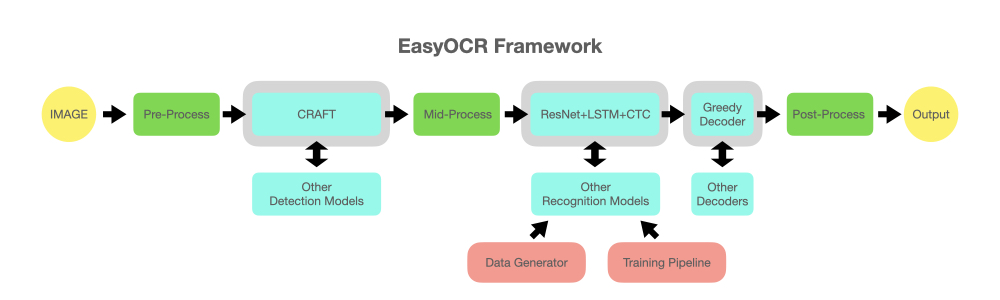
\includegraphics[scale=0.4]{obrazky/easyocr_framework.jpeg}
    \caption{Diagram of EasyOCR pipeline. Grey slots are placeholders for models. The mentioned models are the ones used as default. \cite{easyocr2}}
    \label{img:easyocrPipeline}
\end{figure}

\subsection{Keras-ocr}

keras-ocr is a python library used for detecting and recognizing text in images created by Fausto Morales. It works with variety of languages and with different writing scripts. It allows computing on CPU as well as on GPU.  It unites the CRAFT text detection model and an implementation in Keras python library of CRNN for recognizing text, worth mentioning this is a different implementation of CRNN than in EasyOCR.\cite{keras-ocr1}

On the official website\footnote{\url{https://pypi.org/project/keras-ocr/}} of the package there is a comparison of this method with two other OCR APIs -- Google Cloud Vision and AWS Rekognition. Their performance was tested on 1,000 images from the COCO-Text validation set using a basic pretrained model of each method. None of the investigated methods Michalovice, 293 01 Mlada Boleslavperformed poorly; however, AWS Rekognition had the worst precision and recall results. Google's method and keras-ocr has similar results. It is important to mention that no tuning parameters were used in any of these methods. Another candidate for comparison was Tesseract but it performed on very badly on given data, most likely due to the fact that Tesseract is suitable for scanned documents rather than for photos of real life scenery and objects with text. \cite{keras-ocr1}

CRAFT already provides a pretrained model which can be used directly without modification for text detection or it is used as initial model for training a new model on new data. This model was trained on three datasets (SynthText, IC13, IC17) and supports English and multi language text detection. \cite{craft1}
Similarly for recognition, CRNN also has a pretrained model  This model was trained on the synthetic word dataset which consists of 9 million images with vocabulary of 90K English words. \cite{synth}
To use these models in the keras-ocr library one either doesn't specify anything and use the defaults, or pass the value \texttt{clovaai-general} for the CRAFT pretrained model or \texttt{kurapan} for the CRNN model.

Keras-ocr offers preprocessing for four public datasets though any text image dataset can be examined using this tool. These four datasets are: BornDigital dataset, COCO-Text dataset, ICDAR 2013 dataset, ICDAR 2019 dataset (only Latin-only scripts).\cite{keras-ocrDocu}


\subsection{Google Cloud Vision}

Google Cloud Vision is software from Google which consist of two products: AutoML Vision and Vision API. Vision API detects objects, faces and text from images with already pretrained model. With AutoML Vision user can train custom model from own data. It has free and paid version with a GUI.\cite{google1}
% @misc{google1, title={Vision AI | derive image insights via ML &nbsp;|&nbsp; cloud vision API &nbsp;|&nbsp; google cloud}, url={https://cloud.google.com/vision/}, journal={Google}, publisher={Google}} 
API for python

\subsection{Other}

\subsubsection{AWS Rekognition}

% \chapter{Datasets}

\section{Synthetic datasets}
\section{Scene text image datasets}
\section{Wien TU dataset}


\chapter{Functions description}

In this chapter functions used in testing scripts are shown and briefly described. Note that docstrings of functions were omitted as they provide similar information as the descriptions, but in a shorter version.                                                    
\begin{lstlisting}[caption=]

\end{lstlisting}

The function \tn{}


% -------------------------- XML parsing -------------------------- 
\subsection*{Functions for extracting ground truth}

I created the following functions in order to extract ground truth information from  text files -- in most cases XML files. Each dataset unfortunately uses a different form of annotations. The styles differ in order of data, tag names, even in type of the recorded data (sometimes individual characters and their position is written or information about curvature). For XML parsing I utilized the The ElementTree XML API, which is imported as xml.etree.ElementTree.

\begin{lstlisting}[caption=read\_gt\_ctw\_test]
def read_gt_ctw_test(data, scaling_ratio=1):
    """
    SCUT-CTW1500 dataset (test labels parser)
    Returns ground truth in a tuple - first contains word (string), 
    second coordinates (array with left top xy coordinate and right bottom coor).
    If image was previously scaled, one might need to scale also gt coordinates by given ratio.
    """
    # one line = one bounding polygon : list of coordinates, each separated by commas, last is the text inside 
    # there are #### before each text, two additional ## no text recognized


    annotations = []
    with open(data, "r") as file:
        for line in file:
            line = line.rstrip('\n')
            text = line.split("####")
            label = text[-1]
            coordinates = text[0].split(",")[:-1]
            c = [int(i) for i in coordinates]
            minX = min(c[::2])*scaling_ratio
            maxX = max(c[::2])*scaling_ratio
            minY = min(c[1::2])*scaling_ratio
            maxY = max(c[1::2])*scaling_ratio

            bbox_coords = np.array( [[minX, minY], [maxX, maxY]] )
            annotations.append((label, bbox_coords))

    return annotations
\end{lstlisting}

The function \tn{read\_gt\_ctw\_test} reads 




\begin{lstlisting}[caption=image\_text\_crop]
def image_text_crop(images, filenames, ground_truth, one_file=True, result_folder='./results', skip_longer_than=40):
    # test if there are not more gts than images
    # else the for loop will never get to those exceeding image count
    gt_length = len(ground_truth)
    if len(images) > gt_length:
        images = images[:gt_length]

    if not os.path.isdir(result_folder):
        os.mkdir(result_folder)
    
    all_texts = []
    for i, img in tqdm(enumerate(images)):
        name, ext = os.path.splitext(filenames[i])

        # count regions in one image - used for file naming purposes
        region = 1
        
        for text, bbox in ground_truth[i]:
            if len(text) > skip_longer_than:
                continue
            # select image within coordinates (bbox)
            cropped = img[bbox[0,1]:bbox[1,1], bbox[0,0]:bbox[1,0]]

            # create image file:
            # name in format "original-00region.ext"
            new_name = name + '-' + str(region).zfill(3)

            cv.imwrite(os.path.join(result_folder, new_name + ext), cropped)
            # create  text annotation file(s)
            if one_file:
                all_texts.append(new_name + ext + '\t' + text)
            else:
                # one file for each image with word
                with open(os.path.join(result_folder, new_name + '.gt.txt'), 'w') as f:
                    f.write(text)
            region += 1
    
    if one_file:
        with open(os.path.join(result_folder, 'gt.txt'), 'w') as f:
            for line in all_texts:
                f.writelines(line+'\n')

    return all_texts
\end{lstlisting}

The function \tn{image\_text\_crop} crops and saves images based on bounding boxes provided in ground truth for each text region in an image. This is done for all images in \tn{images} list. Also a text file is created with a corresponding text annotation. The name of the resulted file bears the original image name and a number is attached for each text region. The boolean parameter \tn{one\_file} allows to save ground truths only to a single file. Each line consists then of the name of the cropped image and its annotation. The parameter \tn{skip\_longer\_than} skips ground truths that have more characters than stated, because some OCR tools (such as keras-OCR) does not support long strings.

\begin{lstlisting}[caption=shrink\_all]
def shrink_all(images, width):
    scaled = []
    
    for image in images:
        if image.shape[1] > width:
            ratio = width / image.shape[1]
            height = int(image.shape[0] * ratio)
            new_size = (width, height)  
            scaled.append(cv.resize(image, new_size, interpolation=cv.INTER_AREA))
        else:
            scaled.append(image)
    return scaled    
\end{lstlisting}

The function \tn{shrink\_all} returns a list of resized images to a given width. Images already smaller than width are kept unaffected. The resizing aspects ratio.

\begin{lstlisting}[caption=bounding\_rectangle]
def bounding_rectangle(coordinates):
    x, y = zip(*coordinates)

    return np.array([[int(min(x)), int(min(y))], [int(max(x)), int(max(y))]])
\end{lstlisting}

The function \tn{bounding\_rectangle}
Returns top left and bottom right coordinates of a rectangle, that is circumscribed to a polygon defined by coordinates. These are obtained from predictions for each text region.

% -------------------------- IOU --------------------------  

\begin{lstlisting}[caption=iou]
def iou(pred_box, gt_box):
    # find intersection rectangle coordinates
    x_left = max(pred_box[0][0], gt_box[0][0])
    x_right = min(pred_box[1][0], gt_box[1][0])
    y_top = max(pred_box[0][1], gt_box[0][1])
    y_bottom = min(pred_box[1][1], gt_box[1][1])

    if x_right < x_left or y_bottom < y_top:
        return 0
    
    # compute intersection area
    intersection = (x_right - x_left) * (y_bottom - y_top)

    # compute union area
    pred_area = (pred_box[1][0] - pred_box[0][0]) * (pred_box[1][1] - pred_box[0][1]) 
    gt_area = (gt_box[1][0] - gt_box[0][0]) * (gt_box[1][1] - gt_box[0][1]) 
    union  = pred_area + gt_area - intersection

    # return iou
    return  intersection/union

\end{lstlisting}

The function \tn{iou} computes intersection over union of two bounding boxes, as defined in \ref*{sec:eval}. Both input parameters have to contain top left and bottom right coordinates of a bounding box rectangle.

\begin{lstlisting}[caption=iou\_image]
def iou_image(pred_boxes, gt_boxes):
    ious = []

    # have to determine which prediction bounding box contains same (similar) 
    #  text region as ground truth bounding box
    # find and save the best iou for a prediction box and gt box
    for pred_ind, pred in enumerate(pred_boxes):
        max_iou = 0
        max_ind = 0
        for gt_ind, gt in enumerate(gt_boxes):
            iou_value = iou(pred, gt)
            if (iou_value > max_iou):
                max_iou = iou_value
                max_ind = gt_ind

        # match words from prediction and ground thruth (indeces)     
        ious.append((max_iou, pred_ind, max_ind))

    return ious

\end{lstlisting}

The function \tn{iou\_image} computes intersection over union for all text regions in one image.
Each parameter shall contain a list of two coordinates - (top left, bottom right) of a bounding box rectangle.
Returns a list of tuples - each tuple consists of the highest iou value (thus having the biggest overlap), the index of predicted bounding box and  the index of ground truth bounding box. The indeces are taken from the given lists of bounding boxes or ground truths belonging to one particular image.

\begin{lstlisting}[caption=group\_text]
def group_text(lst):
    grouped = []
    key = lambda x: x[2]

    for k, g in itertools.groupby(sorted(lst, key=key), key):
        list_data = list(zip(*g))
        grouped.append((sum(list_data[0]), list_data[1], k))

    return grouped
\end{lstlisting}

The function \tn{group\_text} is a utility function for matching corresponding strings in a list. The list that is passed as an argument is a list of tuples of IOUs returned from the function \tn{iou\_image}. First for each ground truth bounding box, which is determined by the ground truth index (in this case the third element of the tuple) and it is used as a key. The returned tuple consists of a sum of IOUs, a list of indeces of predicted bounding boxes and ground truth index.

% -------------------------- Text Comparision -------------------------- 


\begin{lstlisting}[caption=compare\_text\_cer]
def compare_text_cer(text, special_characters=False, case_sensitive=False, spaces=True, split=True):
    text_gt, text_pred = text
    # remove special characters and case sensitivity if necessary
    if not spaces:
        text_gt = "".join(char for char in text_gt if (char.isalnum()))
        text_pred = "".join(char for char in text_pred if (char.isalnum()))
    elif not special_characters:
        text_gt = "".join(char for char in text_gt if (char.isalnum() or char.isspace()))
        text_pred = "".join(char for char in text_pred if (char.isalnum() or char.isspace()))
    if not case_sensitive:
        text_gt = text_gt.lower()
        text_pred = text_pred.lower()
    
    corresponding_words = []

    if split:
        words_gt = text_gt.split(" ")
        words_pred = text_pred.split(" ")

        # list of words that are corresponding (based on levenshtein distance)
        # and cer value. (=tuple of three elements)
        # for every predicted word find its corresponding gt wordle
        for word_pred in words_pred:    
            min_dist = (1000, (0, 0))
            min_gt_word = ""                  
            for word_gt in words_gt: 
                l_dist = levenshtein_distance(word_gt, word_pred)
                if l_dist[0] < min_dist[0]:
                    min_dist = l_dist
                    min_gt_word = word_gt
            # count normalized cer (the result will be from 0 to 1), 1 is the worst
            # for computation we devide Levenshtein dist. by sum 
            # of the length of the word and count of insertions performed
            if len(min_gt_word) > 0 and len(word_pred) > 0:
                cer = min_dist[0] / (len(min_gt_word) + min_dist[1][2])
            else:
                cer = 1
            corresponding_words.append((min_gt_word, word_pred, cer))

        # no split of words    
    else:
        l_dist = levenshtein_distance(text_gt, text_pred)

        if len(text_gt) > 0 and len(text_pred) > 0:
            cer = l_dist[0] / (len(text_gt) + l_dist[1][2])
        else:
            cer = 1
        corresponding_words.append((text_gt, text_pred, cer))

    return sorted(corresponding_words)
\end{lstlisting}

The function \tn{compare\_text\_cer} returns a sorted list of corresponding words. Each pair of corresponding words is represented as a tuple of ground truth string, predicted string and a CER value. The first parameter have to be a tuple of a single ground truth string and a predicted string. The argument \tn{special\_characters} ignores all characters except alphanumeric characters and space when \tn{False}. This is applied to both predicted and ground truth strings. When the argument \tn{case\_sensitive} is \tn{False} then all texts are set to lowercase. The \tn{spaces} parameter allows only alphanumeric characters and all spaces are removed. The last one of arguments is \tn{split} and it is used optionally depending on the OCR engine and on dataset. When \tn{True}, strings from ground truth and prediction are split with space used as a separator. Then the Levenshtein distance is computed for each pair of ground truth and predicted word. The best one is chosen for each predicted word and returned together with the two closest words. In case of no split, the Levenshtein distance is computed directly for the strings in the original tuple \tn{text}. It is recommended to use split when the OCR model tends to detect words that belongs to each other as separate words and ground truth marks them as a text line with multiple words. Or when ground truth is one-word and model predicts strings with multiple words together.

The function \tn{levenshtein\_distance} computes the Levenshtein distance (definition can be found in section \ref*{sec:eval}). The implementation is taken from a console application called xer. The code is available from \url{https://github.com/jpuigcerver/xer/blob/master/xer}. It returns a tuple of counts of the three performed operations --  substitution, deletion, insertion.

% -------------------------- Final Visualisation -------------------------- 
\begin{lstlisting}[caption=plot\_results]
def plot_results(image, ground_truth, predicted, size=15):
    # Create figure and axes
    figure, ax = plt.subplots(figsize=(size, size))

    # Display the image
    ax.imshow(cv.cvtColor(image, cv.COLOR_BGR2RGB), cmap=plt.get_cmap('gray'))
    ax.axis('off')

    for label, bbox  in ground_truth:
        topleft = bbox[0]
        height = bbox[1,1] - bbox[0,1]
        width = bbox[1,0] - bbox[0,0]

        # create and add rectangle
        rect = patches.Rectangle((topleft), width, height, linewidth=1, edgecolor='g', facecolor='none')
        ax.add_patch(rect)

        # add labels
        ax.text(topleft[0]+width, topleft[1],label,verticalalignment='top', color='g',fontsize=13, bbox=dict(facecolor='g', alpha=0.2, edgecolor='g'))

    for label, bbox  in predicted:
        topleft = bbox[0]
        height = bbox[1,1] - bbox[0,1]
        width = bbox[1,0] - bbox[0,0]

        # create and add rectangle
        rect = patches.Rectangle((topleft), width, height, linewidth=1, edgecolor='r', facecolor='none')
        ax.add_patch(rect)

        # add labels
        ax.text(topleft[0]-2, topleft[1]-5,label,verticalalignment='top', color='r',fontsize=13, bbox=dict(facecolor='r', alpha=0.2, edgecolor='r'))
    
    # smaller white borders
    plt.subplots_adjust(left=0, bottom=0.1, right=1, top=0.9, wspace=0, hspace=0)

    return plt 
\end{lstlisting}

The function \tn{plot\_results} returns a plot with an image and both predicted and ground truth bounding boxes 
and corresponding labels. The ground truths are marked with green color and predictions with red. Objects are drawn using the package matplotlib.

\begin{lstlisting}[caption=]

\end{lstlisting}

The function \tn{}
\chapter{Results}
\label{ch:results}
In this chapter achieved results are presented. I tested each method on four datasets as described in chapter \ref{ch:sw} and \ref{ch:testing}. Next I will shortly described possible setups of each of the three methods I used in the experiments. It will be  followed by discussion of the results of test divided into sections by the four datasets.
I have divided the experiments by the four datasets and made comparisons. Prediction methods were examined with a different setting of parameters where possible.


\subsection*{EasyOCR}
I used the version 1.5.0 of the EasyOCR python package. The experiments were run using a GPU. I used two different settings for EasyOCR engine -- the basic one which tends to detect and recognize text as single word objects and the second setting merges close words together creating text lines of words that belong together.

\subsection*{Keras-OCR}
The keras\_ocr-0.9.1 package for Python was used in experiments. It was necessary to compute the predictions on GPU, due to the limited GPU on Google Colab and the size of the images needed to be processed one by one although Keras allows to process images in batches. Keras-OCR predictions are case insensitive, because the default model does not support uppercase letters. I trained the Keras recognition model on SCUT-CTW1500 dataset (on the one thousand training images), first a trained the default model with lower case alphabet, then with the same alphabet and a space character and finally with uppercase letters and a set of special characters. In the results discussion it will be shown that after training the model does not offer better results than the original model. THe original model is already very successful and was well trained on much larger datasets.

Each of the training took about an hour on Google Colab GPU. I set 100 epochs and an early stopping based on the value of validation loss. The validation data were taken from the train data as 20\% of the whole training part. First the I used early stopping after 10 non decreasing values, then after 30, but in both cases the model could not get any better than 14\% validation loss.

% graph

\subsection*{Tesseract}
The version of Tesseract installed on Google Colab is tesseract 4.0.0-beta.1 with leptonica-1.75.3, which means that the LSTM network is available. For testing I used the OCR Engine mode (OEM) 3, that is Legacy + LSTM engines. As for Page segmentation modes (PSM) I used numbers 3, 4, 6, 8 and 11, which are "Fully automatic page segmentation, but no OSD. (Default)", "Assume a single column of text of variable sizes.",  "Assume a single uniform block of text.",  "Treat the image as a single word." and "Sparse text. Find as much text as possible in no particular order." respectively. I used PSM 3 only initially and dropped it because prediction was strongly inefficient, so it is not included in result statistics. PSM 8 was used for testing Tesseract with CRAFT, because CRAFT crops an image into segments where there is only one word (or a short text line), therefore Tesseract needed to treat the image as a single word. The rest of mentioned PSMs were applied for examining the behavior of pure Tesseract engine. 

\section*{Experiments}

In this section the results of experiments are divided into four parts based on the four datasets used for testing.

In table \ref{Tab:terms} is explanation of terms used in experiments and result discussion.

\begin{table}[!hbt]
    \centering
    \begin{tabular}{|p{2cm}|p{\textwidth-3cm}|}
    \hline
        Term & Explanation \\
    \hline
        split & If there is a split option, it denotes that predicted strings were chopped into individual words separated by spaces. \\
        no split & It means that predicted string was not changed. \\
        tuning & Parameters of the model, other than the default ones, were set to produce better predictions. \\
        psm & Page segmentation mode -- a parameter for Tesseract. \\
    \hline
    \end{tabular}
    \caption{Explanation of terms used in experiments.}
    \label{Tab:terms}
\end{table}

\newpage
\subsection*{Born-Digital}

First, the Born-Digital Images dataset was tested with images in predictions and ground truth were set to be in lowercase and all special characters except for space were removed. There were 13 different testing runs with three tested methods.  In Figure \ref*{Im:resBD} are the results of this testing and in Table \ref*{Tab:resBD} is corresponding information about each run. 

The best CER value was achieved by tuned EasyOCR engine, where no split was done on predicted text (letter D in Fig. \ref*{Im:resBD}). We can see from the graph and table, that EasyOCR and keras-OCR had significantly better results than Tesseract. Also it can be said that tuning of EasyOCR model results in higher both IoU and CER of approximately 20\% more than with basic EasyOCR setup of parameters. Keras-OCR performs similarly with split and no split option and in both cases gives satisfactory results. The best IoU score was equal to $64.6\%$ (letters G and H) and belongs to keras-OCR model. Tuned EasyOCR can get up to $60.3\%$ without tuning $20\%$ lower than that.

When we compare Tesseract with its own detection model and Tesseract with CRAFT tool, we can see that CRAFT increases the CER metric by more than 12\%, however the IoU metric fluctuates for all cases around 50\%. Whether the image is in RGB color scheme or in grayscale has only a little impact on the results, generally it differed only by about 2\%. Same minor difference is when split or no split option is set. If the Otsu thresholding was performed and the image was then binarized, results were worse than when Tesseract itself performs the binarization. Better results were when PSM Tesseract parameter was set to 11 rather then PSM 4. 

{
\begin{figure}[hbtp!]
    \centering
    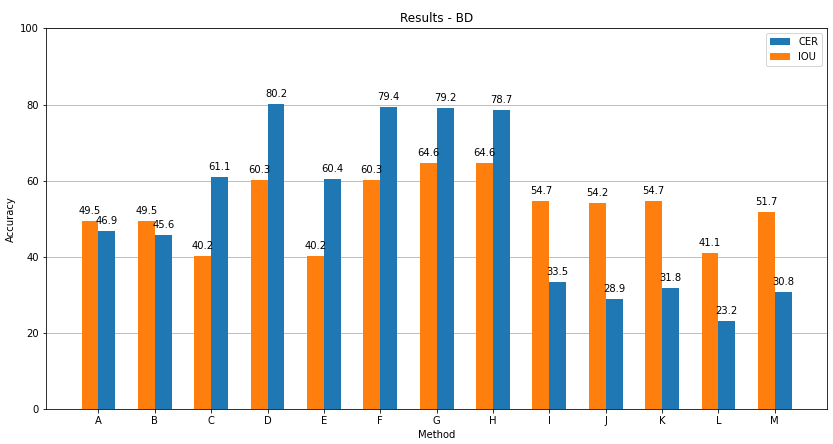
\includegraphics[width=\textwidth]{obrazky/grafy/resBD.png}
    \caption{Results of experiments performed on Born-Digital Images dataset. Information about each method is in Table \ref*{Tab:resBD}.}
    \label{Im:resBD}
\end{figure}
\begin{table}[!hbt]
    \centering
    \begin{tabular}{|l|l|l|}
    \hline
        Key & Method & Properties \\ \hline
        A & tesseract+CRAFT &  no split, psm8\\ 
        B & tesseract+CRAFT &  split, psm8\\ \hline
        C & easyOCR &  no split, no tuning\\ 
        D & easyOCR &  no split, tuning\\ 
        E & easyOCR &  split, no tuning\\ 
        F & easyOCR &  split, tuning\\ \hline
        G & keras-OCR &  no split\\ 
        H & keras-OCR &  split\\ \hline
        I & tesseract & colored, no split, psm11\\ 
        J & tesseract & binary, split, psm11\\ 
        K & tesseract & colored, split, psm11\\ 
        L & tesseract & binary, split, psm4\\ 
        M & tesseract & colored, split, psm4\\ \hline
    \end{tabular}
    \caption{A table of keys for methods and parameters of experiments performed on Born-Digital Images dataset for Figure \ref*{Im:resBD}.}
    \label{Tab:resBD}
\end{table}
}

Next I performed tests with case sensitive option and with special characters included, this option caused a decrease in CER value due to the fact that there are lots of special characters and uppercase words. However, it is good to have a recognizer that can predict more than lowercase strings even at the cost of slightly reducing the accuracy.


\subsection*{SCUT-CTW1500 dataset}
The SCUT-CTW1500 dataset was again first tested with predictions and ground truth were set to be in lowercase and all special characters except for space were removed. 14 different testing were run.  In Figure \ref*{Im:resCTW} are the results of the testing and the corresponding information about each run is in Table \ref*{Tab:resCTW}. 

This time the best CER value ($76.4\%$) was achieved by keras-OCR model, where split was performed on predicted text (letter H in Fig. \ref*{Im:resCTW}). It can be seen from the graph and table, that EasyOCR and keras-OCR had again significantly better results than Tesseract. In testing of CTW1500 dataset this time keras-OCR generally performed better than EasyOCR in CER metric by roughly 10\%. The tuning of EasyOCR model results in lower both IoU and CER of approximately 2\% less than with basic EasyOCR setup of parameters. This might by probably due to the fact that EasyOCR model was trained on data similar to CTW1500 dataset rather then Born-Digital Images dataset keras-OCR performs simlarly with split and no split option and in both cases gives satisfactory results.

The Comparison of Tesseract with its own detection model and Tesseract with CRAFT tool shows that with CRAFT the CER metric increased by almost than 20\% as well as the IoU metric that increased by more than 30\%. Plain Tesseract results are again the worst and are not heavily influenced by color scheme or slight scaling changes. 

\begin{figure}[hbtp!]
    \centering
    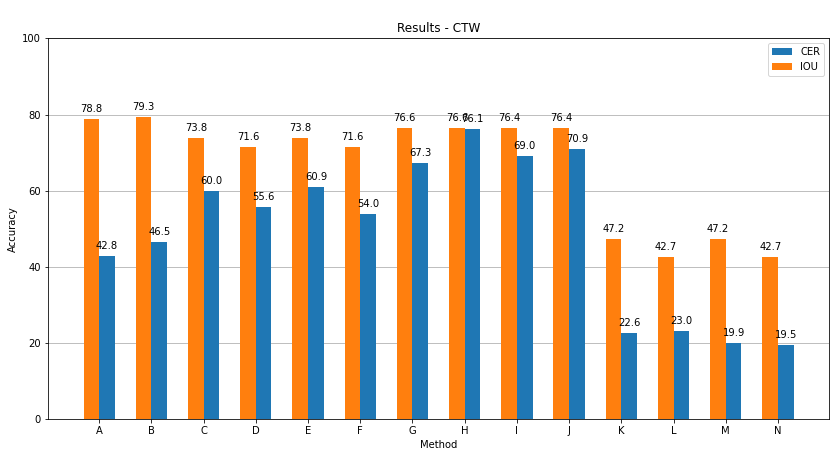
\includegraphics[width=\textwidth]{obrazky/grafy/resCTW.png}
    \caption{Results of experiments performed on CTW dataset. Information about each method is in Table \ref{Tab:resCTW}.}
    \label{Im:resCTW}
\end{figure}
\begin{table}[!ht]
    \centering
    \begin{tabular}{|l|l|l|}
    \hline
        Key & Method & Properties \\ \hline
        A & tesseract+CRAFT & no split \\ 
        B & tesseract+CRAFT & split \\ \hline
        C & easyOCR & nosplit, notuning \\ 
        D & easyOCR & no split, tuning \\ 
        E & easyOCR & split, notuning \\ 
        F & easyOCR & split, tuning \\ \hline
        G & keras-OCR & original image width, no split \\ 
        H & keras-OCR & original image width, split \\ 
        I & keras-OCR & original image width, split, trained spaces \\ 
        J & keras-OCR & original image width, split, trained \\ \hline
        K & tesseract & 3000px image width, no split \\ 
        L & tesseract & color, no split, psm11 \\ 
        M & tesseract & split, psm11\\ 
        N & tesseract & color, split, psm11 \\ \hline
    \end{tabular}
    \caption{A table of keys for methods and parameters of experiments performed on SCUT-CTW1500 dataset for Figure \ref{Im:resCTW}.}
    \label{Tab:resCTW}
\end{table}

\subsection*{KAIST Scene Text Database}

Testing of performance of the three methods on KAIST dataset with case insensitivity and no special characters was done in 22 different runs. Eight of them were on KAIST bitmap images, as these images do not have a misleading background the results are significantly better than on original photographes. The results can be seen in Figure \ref*{Im:resK} and the corresponding information is in Table \ref*{Tab:resK}. 
The best results on the bitmap images part of KAIST dataset were performed by EasyOCR dataset with no splitting and CER value is $82.2\%$ high (letter B in Fig. \ref*{Im:resK}). This method with the same setup is also best with KAIST dataset unedited photographs. Due to the character of the dataset for all cases the no split option is distinctly better. 

Keras-OCR had slightly lower values of CER than EasyOCR and IoU values are even lower by generally 15\%. Still it is by 20\% higher than results of plain Tesseract and comparable with Tesseract and CRAFT combination. Tesseract had this time best but still way too low results with PSM 6. PSM 4 led to CER value as low as 18\%. Color scheme did not have a distinguishable impact on the results.
 
\begin{figure}[hbtp!]
    \centering
    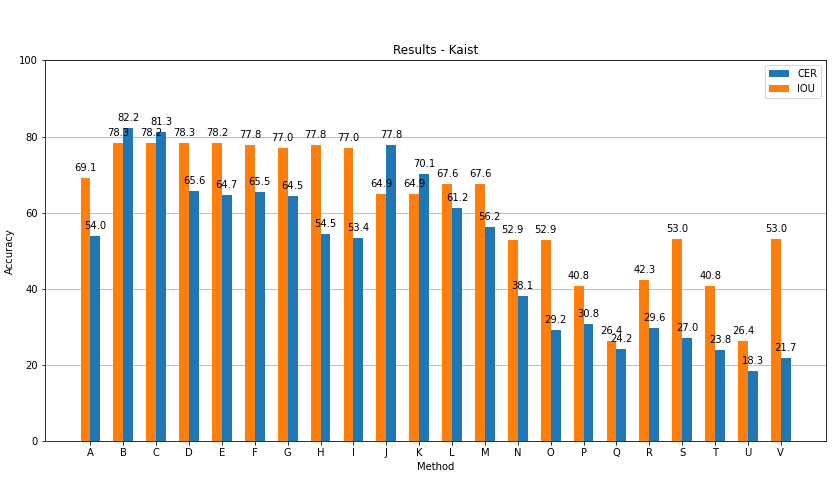
\includegraphics[width=\textwidth]{obrazky/grafy/resKaist.png}
    \caption{Results of experiments performed on KAIST Scene Text Database. Information about each method is in Table \ref{Tab:resK}.}
    \label{Im:resK}
\end{figure}
\begin{table}[!ht]
    \centering
    \begin{tabular}{|l|l|l|}
    \hline
        Key & Method & Properties \\ \hline
        A & tesseract+CRAFT & no split \\ \hline
        B & easyOCR & bmp, no split, no tuning \\ 
        C & easyOCR & bmp, no split, tuning \\ 
        D & easyOCR & bmp, split, no tuning \\ 
        E & easyOCR & bmp, split, tuning \\ 
        F & easyOCR & no split, no tuning \\ 
        G & easyOCR & no split, tuning \\ 
        H & easyOCR & split, no tuning \\ 
        I & easyOCR & split, tuning \\ \hline
        J & keras-OCR & bmp, no split \\ 
        K & keras-OCR & bmp, split \\ 
        L & keras-OCR & no split \\ 
        M & keras-OCR & split \\ \hline
        N & tesseract & bmp, no split, psm11 \\ 
        O & tesseract & bmp, split, psm11 \\ 
        P & tesseract & colored, no split, psm11 \\ 
        Q & tesseract & colored, no split, psm4 \\ 
        R & tesseract & colored, no split, psm6 \\ 
        S & tesseract & no split, psm11 \\ 
        T & tesseract & colored, split, psm11 \\ 
        U & tesseract & colored, split, psm4 \\ 
        V & tesseract & split, psm11 \\ \hline
    \end{tabular}
    \caption{A table of keys for methods and parameters of experiments performed on KAIST Scene Text Database for Figure \ref{Im:resK}.}
    \label{Tab:resK}
\end{table}



% Training took one hour and stopped after 57 epochs ,10.979148864746094,20.5778751373291. Continued training.

% trained no spaces 
% [[('bruno', 'brung', 0.2)],
%  [('optique', 'ortinu', 0.42857142857142855),
%   ('optique', 't', 0.8571428571428571)],
%  [('promotion', 'mgtioa', 0.5555555555555556),
%   ('promotion', 'rro', 0.7777777777777778)],
%  [('la', 'bne', 1.0),              ('paire', 'paite', 0.2)]]
%  [[('panns', 'aine', 0.6)],
%  [('1958', '1953', 0.25), ('since', 'simce', 0.2)],
%  [('food', 'food', 0.0), ('real', 'rea', 0.25)]]
%   ('la', 'loz', 0.6666666666666666),
%                 ('paire', 'paite', 0.2)]]
%                 [[('panns', 'aine', 0.6)],
%                 [('1958', '1953', 0.25), ('since', 'simce', 0.2)],
%                 [('food', 'food', 0.0), ('real', 'rea', 0.25)]]


% CTW
% training with special chars case insensitive no special split
% [[('bruno', 'bruns', 0.2)],
%  [('optique', 'optoue', 0.2857142857142857), ('optique', 'srss', 1.0)],
%  [('promotion', 'bre', 0.8888888888888888),
%   ('promotion', 'motion', 0.3333333333333333)],
%  [('2eme', 'enne', 0.75), ('la', 'le', 0.5), ('la', 'salls', 0.8)]]

%  s no splitem 60 to je fakt malo ani ne v grafu

%  velka pismena a znaky
%  [[('BRUNO', 'BRUNS', 0.2)],
%  [('OPTIQUE', 'OPTOUE', 0.2857142857142857), ('OPTIQUE', 'SRSS', 1.0)],
%  [('PROMOTION', 'BRE', 0.8888888888888888),
%   ('PROMOTION', 'MOTION', 0.3333333333333333)],
%  [('2eme', 'enne', 0.75), ('La', 'Le', 0.5), ('La', 'Salls', 0.8)]]

%  [[('DOUGLASTON', 'BOUGLASTON', 0.1)],
%  [('E-313', 'E313', 0.2)],
%  [('L164', 'Lbl6w', 0.6)],
%  [('F.D.N.Y.', 'EDNY', 0.625)]]

% BD

% nula

% [[('flying', 'tying', 0.3333333333333333)],
%  [('today', 'todoy', 0.2)],
%  [('means', 'eons', 0.4)],
%  [('vueling', 'VUelnng', 0.42857142857142855)],
%  [('GET', 'GET', 0.0)],
%  [('', 'AVAY.', 1)],
%  [('1.000.000', '1.000.000', 0.0)],
%  [('SEATS', 'SEATS', 0.0)],
%  [('FROM', 'FRON', 0.25)],
%  [('30€', '303', 0.3333333333333333)],
%  [('Book', 'BOOK', 0.75)],
%  [('now!', 'nowi', 0.25)]]

% Case sensitivity


% when default model is used and special characters and case sensitivity of ground truth labels is observed CER accuracy reaches only less than thirty percent. 

\newpage

\subsection*{Vienna City Poster Dataset}

The Vienna City Poster Dataset was detected and recognized with the same method as previously mentioned datasets. Even though the dataset has only a little over 250 images, it is that large that the RAM size available in Google Colab struggled to work with the dataset as whole I had to split the dataset into two parts and perform computations on them separately. Then I combined the corresponding results. Specifically, the first group included first 123 images, the second the rest, where data were sorted by name of the files.

I used different parameters that can be set in each method. However, in the result table \ref{Tab:resV} and graph \ref*{Im:resV} I selected only the best ones within each method. Thus the results contains     thirteen CER and IoU values. In the featured results for all cases except one I tested only alphanumeric characters without the sensitivity to their case.

Due to the fact that this dataset is mainly in German language, in all models I set German as the language that is to be predicted. The defualt was English for all models. I implemented possible language correction which takes common syllables that appear in German. The function is described in \ref{lst:correctgerman}. For some predictors these corrections were not necessary and predicted similarly without them. 

\begin{figure}[hbtp!]
    \centering
    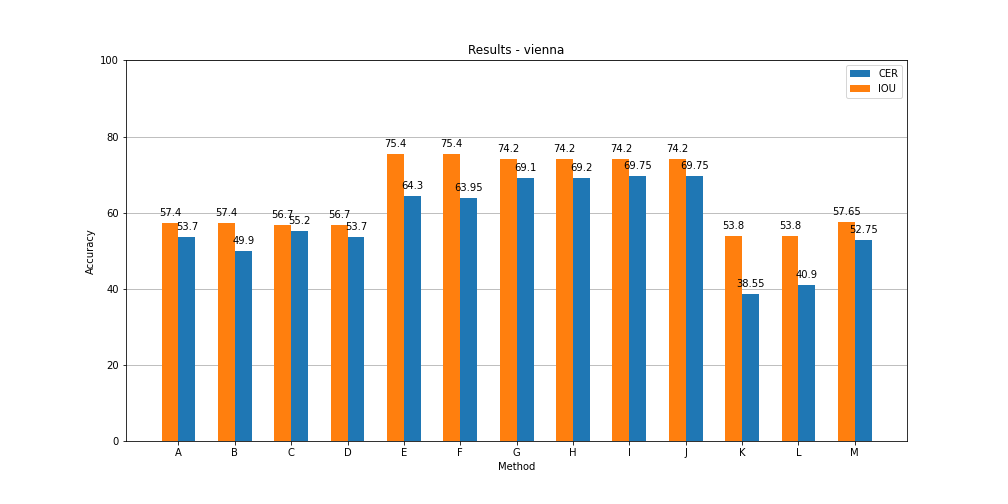
\includegraphics[width=\textwidth]{obrazky/grafy/resvienna.png}
    \caption{Results of experiments performed on Vienna City Poster Dataset. Information about each method is in Table \ref{Tab:resV}.}
    \label{Im:resV}
\end{figure}

\begin{table}[!ht]
    \centering
    \begin{tabular}{|l|l|l|}
    \hline
        Key & Method & Properties \\ \hline
        A & Tesseract+CRAFT & split \\
        B & Tesseract+CRAFT & case sensitive, includes special characters, split \\ \hline
        C & easyOCR & no split, no tuning, correction\\
        D & easyOCR & no split, no tuning, no correction \\
        E & easyOCR & no split, tuning, correction\\
        F & easyOCR & split, tuning, correction" \\ \hline
        G & keras-OCR & no split, correction" \\
        H & keras-OCR & no split, no correction" \\ 
        I & keras-OCR & split, correction" \\ 
        J & keras-OCR & split, no correction" \\ \hline
        K & tesseract & no split, psm11" \\ 
        L & tesseract & split, psm11" \\ 
        M & tesseract & split, psm4" \\ \hline
    \end{tabular}
    \caption{A table of keys for methods and parameters of experiments performed on Vienna City Poster dataset dataset for Figure \ref{Im:resV}.}
    \label{Tab:resV}
\end{table}

The best results were obtained by EasyOCR and keras-OCR. The highest IoU score is equal to $75.4\%$ and it belongs to EasyOCR method with its parameters tuned to create tighter bounding boxes than pure EasyOCR (letters E and F in Fig. \ref{Im:resV}). In this case the CER values ranged around $64\%$ and correction for German language was involved.
Keras-OCR is responsible for the highest CER value -- $69.75\%$, for both with and without correction. Though the IoU value is sligtly smaller than the best one -- $74.2\%$ (letters G-J). 

As EasyOCR is able to predict also special characters and can be sensitive to case in its result I tested the two best settings (letters E and F) with this option. The CER scores lowered by approximately $3.5\%$. Which means that even with case sensitivity and more characters the model can give very good results. In contrast with keras-OCR which cannot predict special characters and ignores text case without training. To gain this aibility, I trained the keras-OCR model on the Vienna Dataset. I used the the second group of the dataset data as a training images and the first 123 images as testing ones. After seventeen minutes, which accords with twenty epochs, the training ended, because last ten epochs the validation loss stopped decreasing. Unfortunately the trainind dataset would need more data. After tests the IoU score was equal to $73.2\%$ and CER score was $72.1\%$ without my language corrections and with split applied to predictions. These numbers shows that keras-OCR outperforms other models in both with simple characters and with special characters.

Tesseract (letters K-M in Fig. \ref*{Im:resV}) performance, similarly as with other tested datasets, was the worst. Usually the problem was caused by poor detection of the individual words. Very often objects were detected as letters, this happens when the PSM 11 was used. This eleventh option --  find as much text as possible in no particular order -- sounds ideal, because in the posters the text mainly does not keep an order and is present in various locations, orientations and sizes. CER values ranged around $40\%$. However, PSM 4, which assumes a single column of text of variable sizes, performed better with alike accuracy as Tesseract recognizer with CRAFT detector or as untuned EasyOCR, CER values reached neraly up to $53\%$. This comparision was unrealistic for scene text datasets.

When CRAFT package was used as a detector and cropped detected words were sent to Tesseract recognizing tool and treated as a single word (PSM 8). Then the CER score was equal to $53.7\%$ (letters A and B in Fig. \ref*{Im:resV}).


% ---------------------------- Result Conclusion --------------------------------------
\section*{Result Conclusion}

The previous section contains a discussion over achieved results. From this discussion it can be concluded that keras-OCR and EasyOCR have the best results for all datasets. The CER score fluctuates between $65\%$ and $80\%$. The upper boundary is very good and the lower also indicates acceptable predictions. The detection statistics, IoU, for these two winning methods is between $63\%$ and $75\%$.

It can also be concluded that Tesseract gave overall the worst results. When performed on scene text image data, it returned CER value usually around $20\%$, on born-digital data results were around $30\%$ and for the most important Vienna dataset it returned values ranging from $38\%$ to nearly $53\%$. However these numbers are still lower than of any other method. When I changed the default detector in Tesseract to CRAFT detection tool, for all datasets the IoU statistics slightly increased and for the CER statistics a significant rise occured. In cases of SCUT-CTW1500 dataset and KAIST Scene Text Database the CER value doubled. A statement can be made regarding the page segmentation mode 11 of Tesseract tool -- PSM 11, used for images where we want to find as much text as possible, causes that Tesseract finds  much more words in the image and mistakes patterns for letters. This causes that a problem when interpreting the metrics. The IoU can falsely increase, because small false bounding boxes can cover parts of ground truth boxes bounding some large unrecognized word.

In \ref*{ch:appendix} there are examples of images selected from the Vienna City Poster Dataset. Predictions of methods and ground truths are displayed on the images can be compared with each other. I also selected in the examples a couple of images with fonts difficult to recognize.

It is important to say that if there was a bigger labeled dataset for testing the methods, the score values would be more precise and the very difficult fonts and images would not have such an impact on the statistics as they did.
\chapter{Conclusion}

As in other image recognition problems context is a key element in optical character recognition. 

When posters and advertisements are considered it is probable that a product name 

!!!!TBC



\bibliographystyle{PhDbiblio-url} 
\bibliography{sources}

% \chapter*{Závěr} % SEM NESAHEJTE!
% \addcontentsline{toc}{chapter}{Závěr} % SEM NESAHEJTE!
%



%%%%%%%%%%%% SEZNAM POUŽITÝCH ZDROJŮ (LITERATURA) %%%%%%%%%%%%
\clearpage  % SEM NESAHEJTE!
\addcontentsline{toc}{chapter}{Bibliography} % SEM NESAHEJTE!

% \input{tex/bibliografie1.tex}
% \bibliographystyle{unsrt}
% \bibliography{bibliografie}


%%%%%%%%%%%% PŘÍLOHY PRÁCE %%%%%%%%%%%%
\newpage % SEM NESAHEJTE!
\addcontentsline{toc}{chapter}{Appendix} % SEM NESAHEJTE!
\appendix % SEM NESAHEJTE!
\label{ch:appendix}


%%%%%%%%%%%% Příloha A (tj. 1. kapitola v rámci příloh) %%%%%%%%%%%%

% \chapter{Obsah přiloženého CD}
\section*{Image Examples of Results}

A selection of images from the Vienna City Poster Dataset is presented, with predictions and ground truth bounding boxes and labels. Red colour is for predictions and green for ground truth. Also I added comments on used method and achieved CER score. Some images are cropped because in the upper part of the picture is no text and results are then better comparable. First I have chosen images with good results and well legible text, then I have chosen images with complicated text for detection and recognition. They are readable by a human but machines might struggle because they remind more of images than letters, or are only half visible and strong contextual information is needed. 

In table \ref{Tab:terms} is explanation of terms used in experiments and result discussion.

%--------balerina image
\subsection*{P-117050}
This image has well readable letters and for all tested models this image was not difficult to read and only minor mistakes occurred.

\begin{figure}[hbtp!]
    \centering
    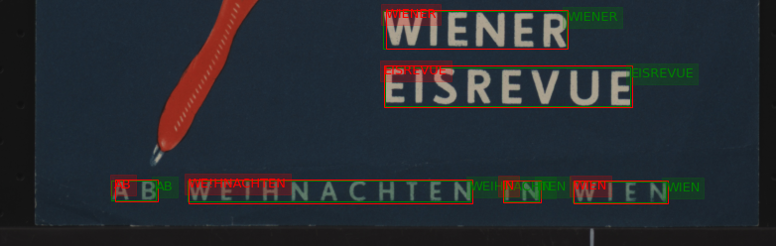
\includegraphics[scale=0.36]{obrazky/plakaty/result_easyOCR_vienna1_split_tuning_special_sensitive-21.png}
    \caption{EasyOCR, tuning on image P-117050}
    \label{Im2:ex:easy}
\end{figure}

\begin{figure}[hbtp!]
    \centering
    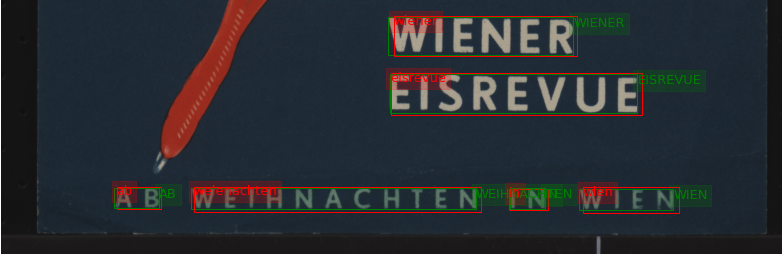
\includegraphics[scale=0.36]{obrazky/plakaty/result_kerasOCR_vienna1_nosplit_nocorrection-21.png}
    \caption{Keras-OCR, untrained on image P-117050}
    \label{Im2:ex:keras}
\end{figure}

\begin{figure}[hbtp!]
    \centering
    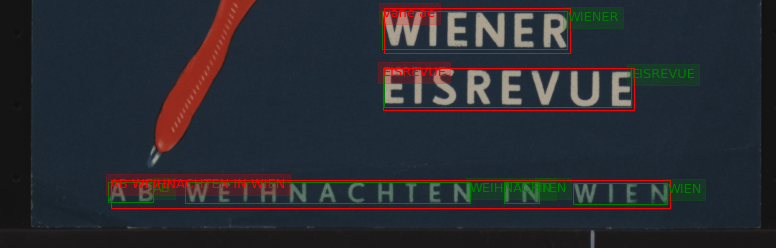
\includegraphics[scale=0.36]{obrazky/plakaty/result_carfttesseract_vienna1_split-21.png}
    \caption{Tesseract+CRAFT on image P-117050}
    \label{Im2:ex:Craft}
\end{figure}

\begin{figure}[hbtp!]
    \begin{subfigure}{\textwidth}
        \centering
        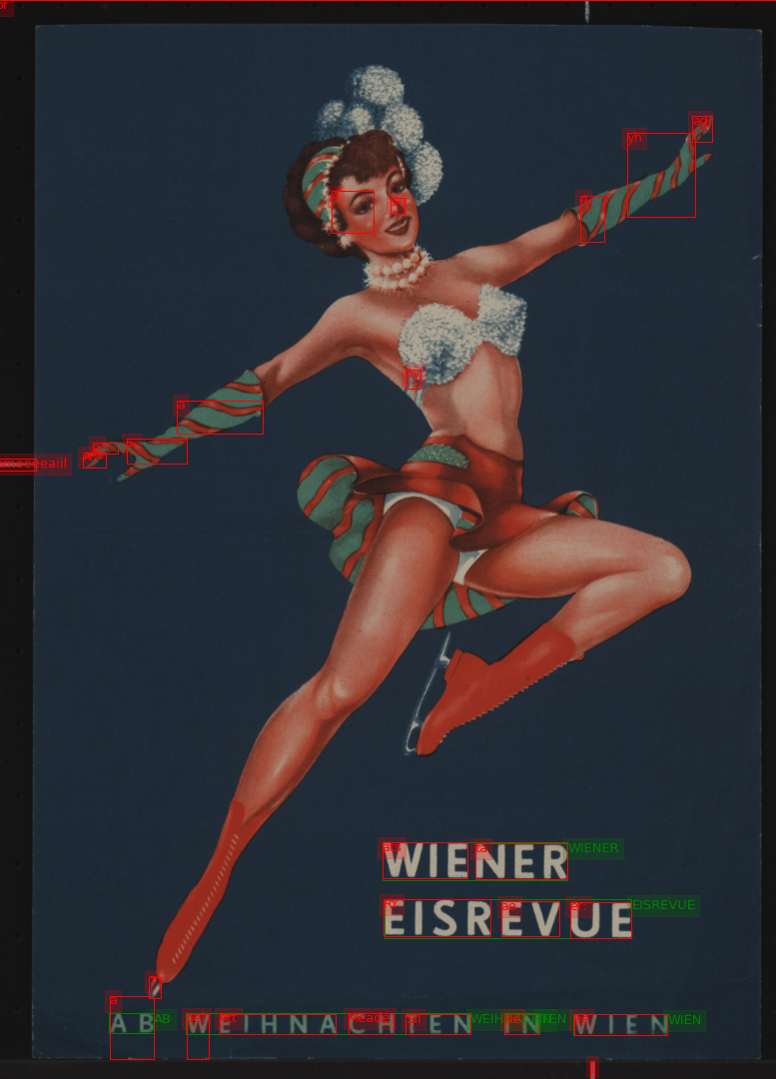
\includegraphics[scale=0.36]{obrazky/plakaty/result_tesseract_vienna1_nosplit_psm11-21.png}
        \caption{PSM 11}
        \label{Im2:ex:tess11}
    \end{subfigure}

    \begin{subfigure}{\textwidth}
        \centering
        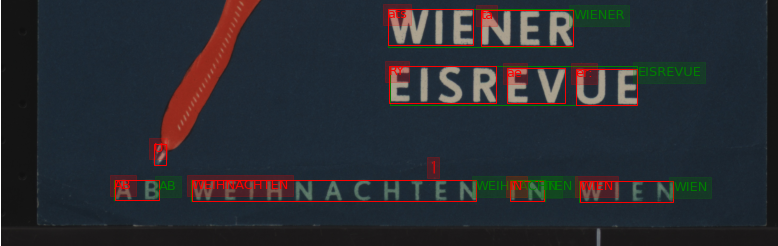
\includegraphics[scale=0.36]{obrazky/plakaty/result_tesseract_vienna1_split_psm4-21.png}
        \caption{PSM 4}
        \label{Im2:ex:tess4}
    \end{subfigure}
    \caption{Tesseract on image P-117050}
    \label{Im2:ex:tess}
\end{figure}


\subsection*{P-2638}

\begin{figure}[hbtp!]
    \begin{subfigure}{\textwidth}
        \centering
        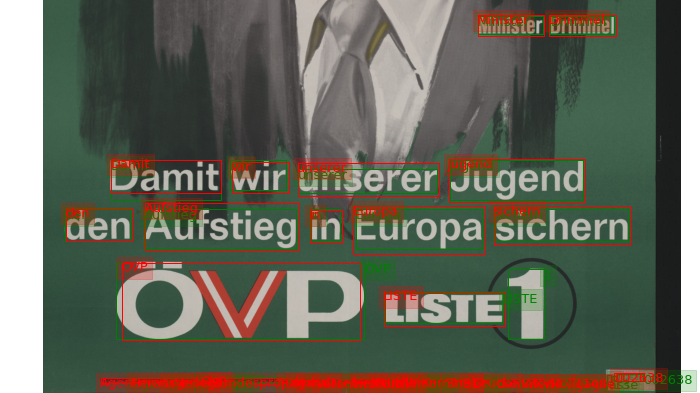
\includegraphics[scale=0.36]{obrazky/plakaty/result_easyOCR_vienna1_split_tuning-91.png}
        \caption{tuning}
        \label{Im1:ex:easytun}
    \end{subfigure}

    \begin{subfigure}{\textwidth}
        \centering
        
\includegraphics[scale=0.36]{obrazky/plakaty/result_easyOCR_vienna1_nosplit_notuning-91.png}
        \caption{no tuning}
        \label{Im1:ex:easy}
    \end{subfigure}
    \caption{EasyOCR on image P-2638}
    \label{Im1:ex:EasyOCR}
\end{figure}

\begin{figure}[hbtp!]
    \begin{subfigure}{\textwidth}
        \centering
        
\includegraphics[scale=0.36]{obrazky/plakaty/result_kerasOCRtrained_vienna1_split-90.png}
        \caption{Keras-OCR, trained}
        \label{Im1:ex:kertr}
    \end{subfigure}

    \begin{subfigure}{\textwidth}
        \centering
        
\includegraphics[scale=0.36]{obrazky/plakaty/result_kerasOCR_vienna1_nosplit_nocorrection-90.png}
        \caption{Keras-OCR}
        \label{Im1:ex:ker}
    \end{subfigure}
    
    \caption{Keras-OCR  on image P-2638}
    \label{Im1:ex:Keras}
\end{figure}


\begin{figure}[hbtp!]
    \centering
    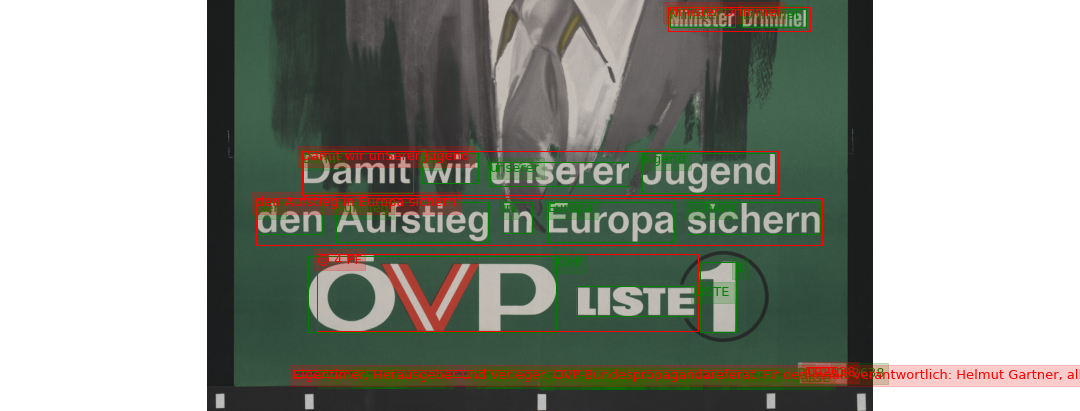
\includegraphics[scale=0.36]{obrazky/plakaty/result_carfttesseract_vienna1_split_special_snesitive-91.png}
    \caption{Tesseract+CRAFT  on image P-2638}
    \label{Im1:ex:craft}
\end{figure}


\begin{figure}[hbtp!]  
    \centering
    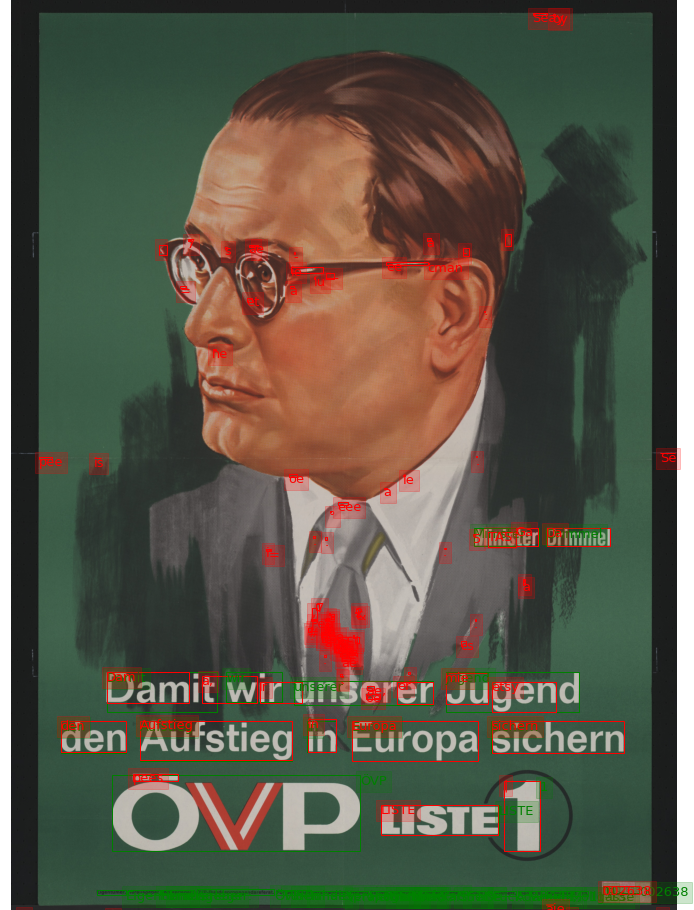
\includegraphics[scale=0.36]{obrazky/plakaty/result_tesseract_vienna1_split_psm11-91.png}
    \caption{Tesseract, PSM 11  on image P-2638. Tesseract found many non existing words and tried to predict them.}
    \l2638abel{Im1:ex:tess11}
\end{figure}

\newpage
\subsection*{P-315617}

\begin{figure}[hbtp!]
    \begin{subfigure}{\textwidth}
        \centering
        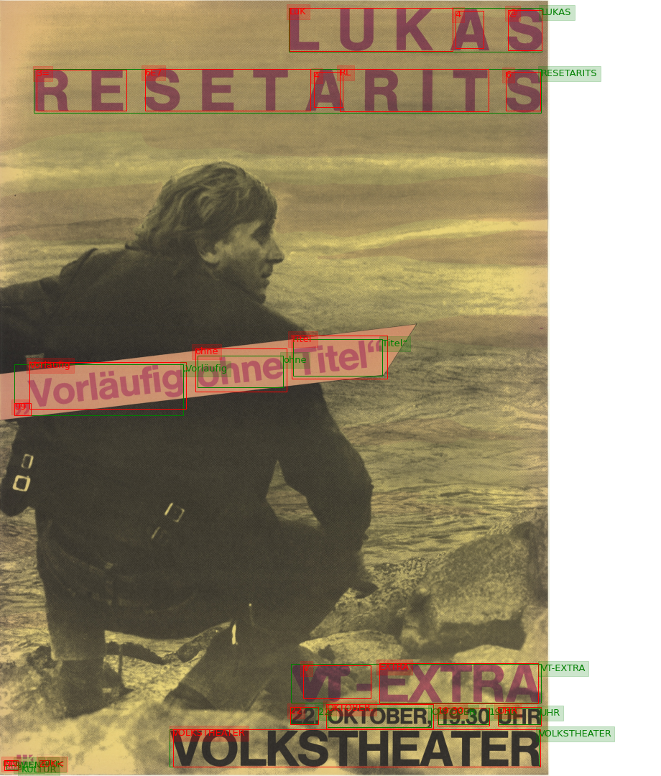
\includegraphics[scale=0.29]{obrazky/plakaty/result_easyOCR_vienna2_nosplit_tuning-83.png}
        \caption{tuning}
        \label{Im3:ex:easytun}
    \end{subfigure}

    \begin{subfigure}{\textwidth}
        \centering
        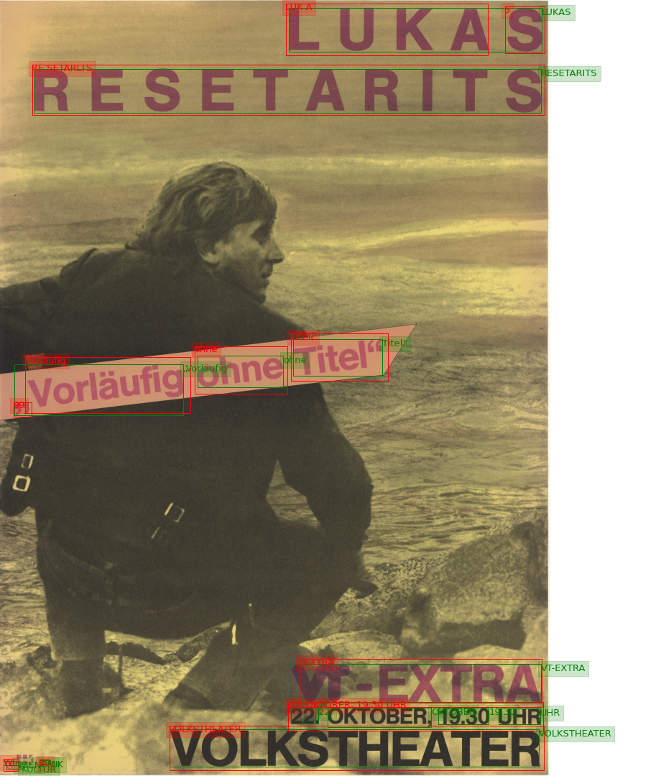
\includegraphics[scale=0.29]{obrazky/plakaty/result_easyOCR_vienna2_nosplit_notuning_nocorrection-83.png}
        \caption{no tuning}
        \label{Im3:ex:easy}
    \end{subfigure}
    \caption{EasyOCR on image P-315617}
    \label{Im3:ex:EasyOCR}
\end{figure}

\begin{figure}[hbtp!]
    \centering
   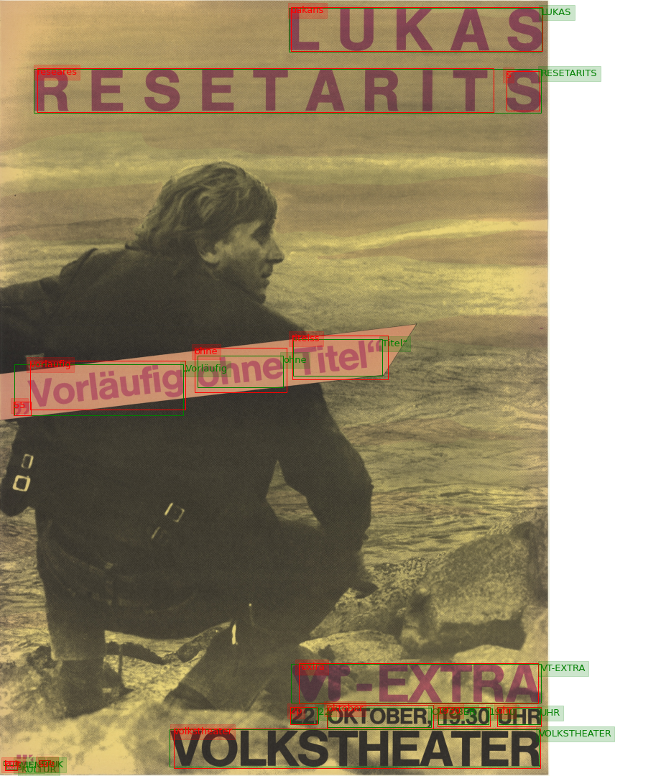
\includegraphics[scale=0.3]{obrazky/plakaty/result_kerasOCR_vienna2_nosplit-83.png}
    \caption{Keras-OCR, untrained  on image P-315617}
    \label{Im3:ex:keras}
\end{figure}

\begin{figure}[hbtp!]
    \centering
    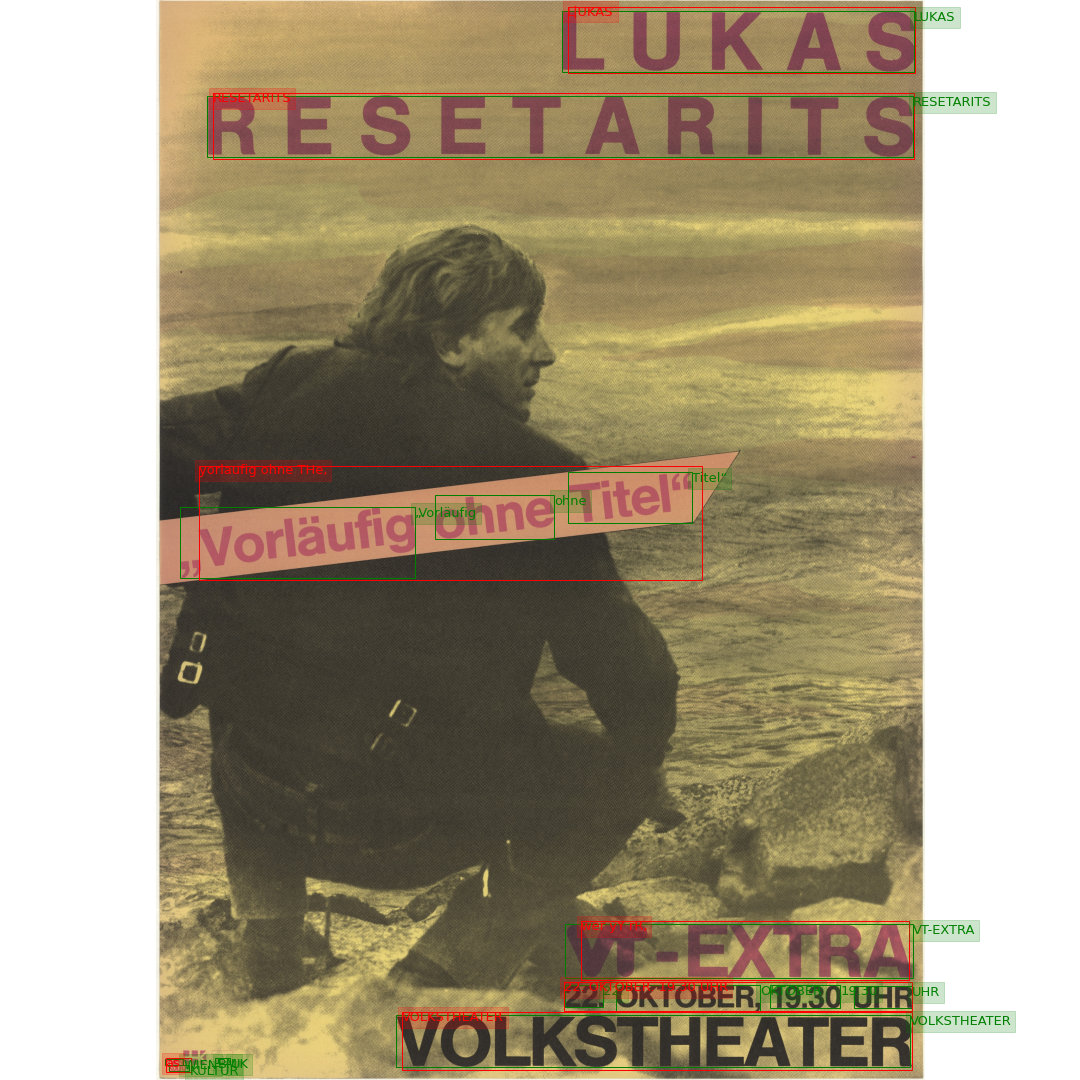
\includegraphics[scale=0.3]{obrazky/plakaty/result_carfttesseract_vienna2_split_special_snesitive-83.png}
    \caption{Tesseract+CRAFT  on image P-315617}
    \label{Im3:ex:craft}
\end{figure}

\begin{figure}[hbtp!]
    \begin{subfigure}{\textwidth}
        \centering
        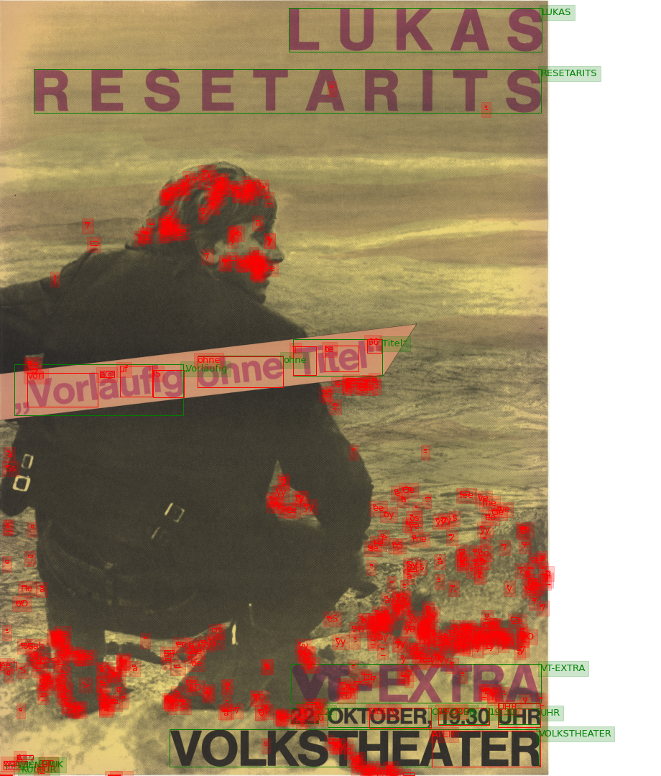
\includegraphics[scale=0.29]{obrazky/plakaty/result_tesseract_vienna2_nosplit_psm11-83.png}
        \caption{PSM 11 on image P-315617. Tesseract found many non existing words and tried to predict them.}
        \label{Im4:ex:tess11}
    \end{subfigure}

    \begin{subfigure}{\textwidth}
        \centering
        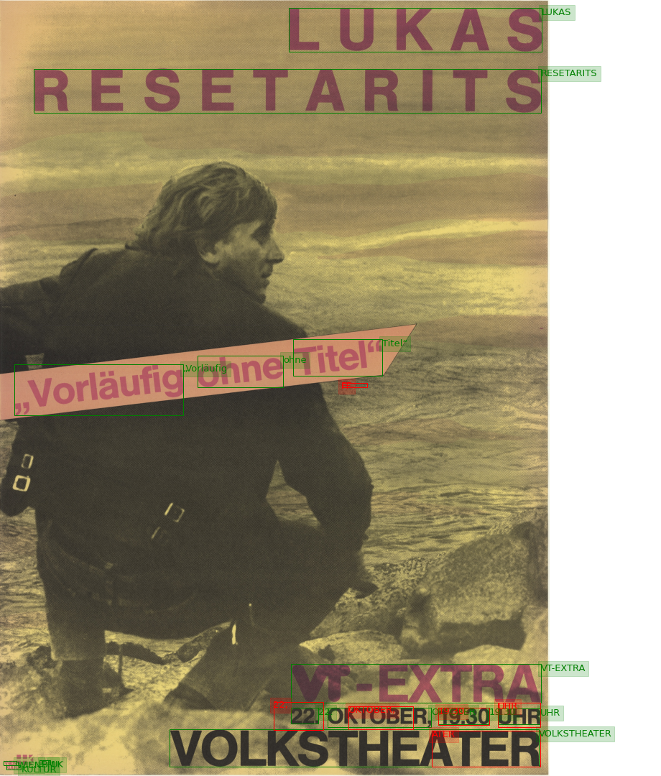
\includegraphics[scale=0.29]{obrazky/plakaty/result_tesseract_vienna2_split_psm4-83.png}
        \caption{PSM 4}
        \label{Im4:ex:tess4}
    \end{subfigure}

    \caption{Tesseract  on image P-315617}
    \label{Im3:ex:tess}
\end{figure}

\newpage
\subsection*{P-236873}
% result_easyOCR_vienna1_split_tuning_special_sensitive-55.png
% result_easyOCR_vienna2_nosplit_notuning_nocorrection-70.png

This image has a text that is supposed to look like northern lights in a night sky and is not easy to read even by humans. None of the models were able to identify the wavy text.

\begin{figure}[hbtp!]
    \begin{subfigure}{0.5\textwidth}
        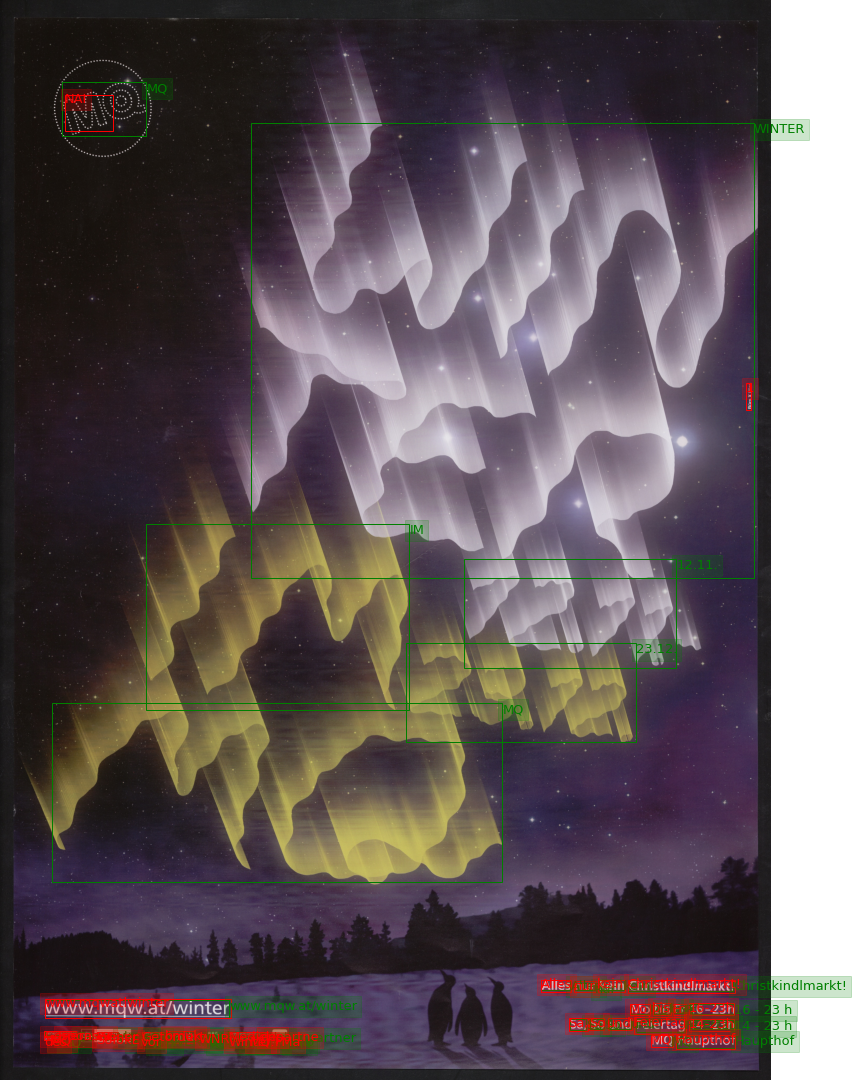
\includegraphics[scale=0.3]{obrazky/plakaty/result_easyOCR_vienna1_split_tuning_special_sensitive-73complecatedP-236873.png}
        \caption{EasyOCR}
        \label{Im4:ex:easy}
    \end{subfigure}
    \begin{subfigure}{0.45\textwidth}
        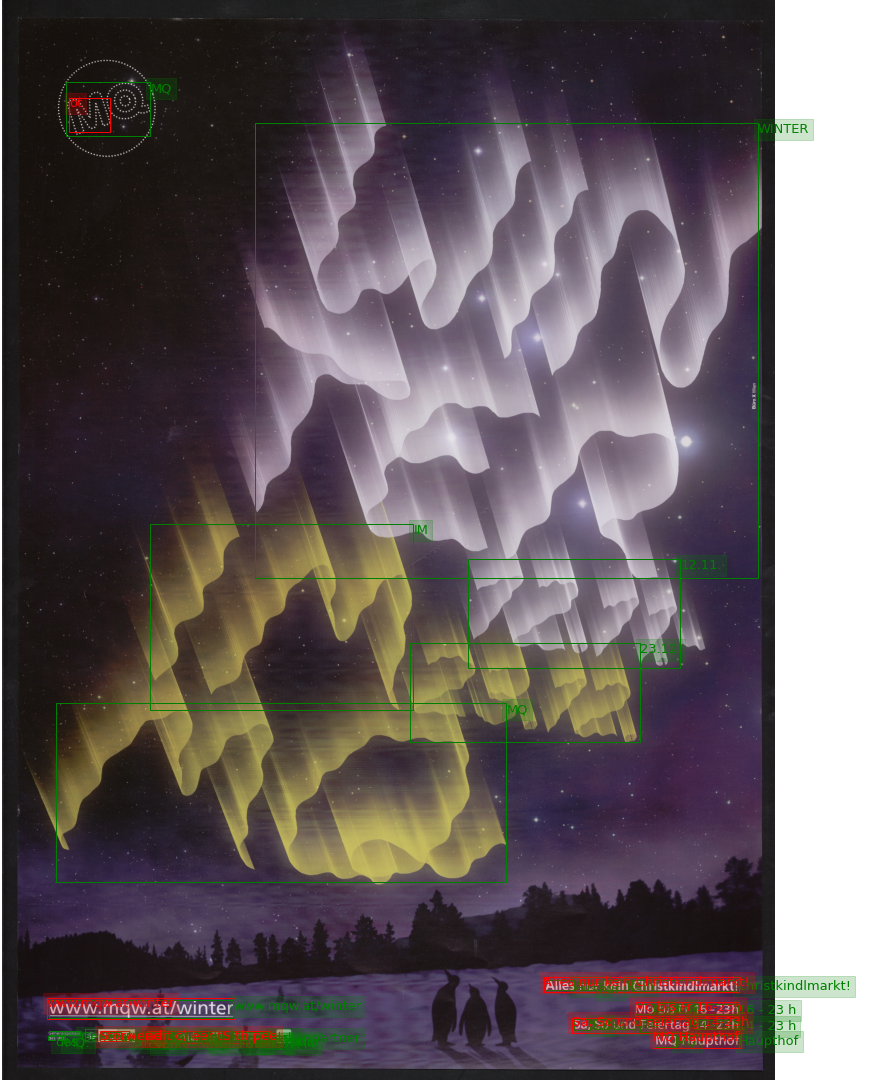
\includegraphics[scale=0.3]{obrazky/plakaty/result_carfttesseract_vienna1_split_special_snesitive-73.png}
        \caption{Tesseract+CRAFT}
        \label{Im4:ex:craft}
    \end{subfigure}

    \caption{Tesseract on image P-236873}
    \label{Im4:ex:compl}
\end{figure}

\newpage
\subsection*{P-229767}
This image is a challenge for the detector and recognizer because there is a large number 10. The height and width of the number is same as the dimensions of the whole image and on top of that the number zero is not completely visible. Then there is curved text, which is also challenging. 

\begin{figure}[hbtp!]
    \centering
    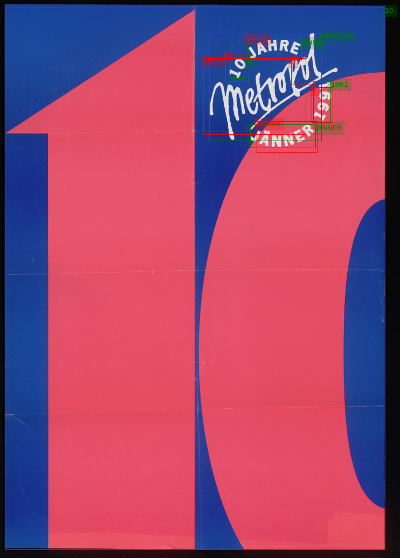
\includegraphics[scale=0.8]{obrazky/plakaty/result_easyOCR_vienna1_split_tuning_special_sensitive-55.png}
    \caption{EasyOCR  on image P-229767}
    \label{Im5:ex:easy}
\end{figure}


\subsection*{P-231248}
This image demonstrates that vertical text is more complicated for the recognizer although it is quite legible.

\begin{figure}[hbtp!]
    \centering
    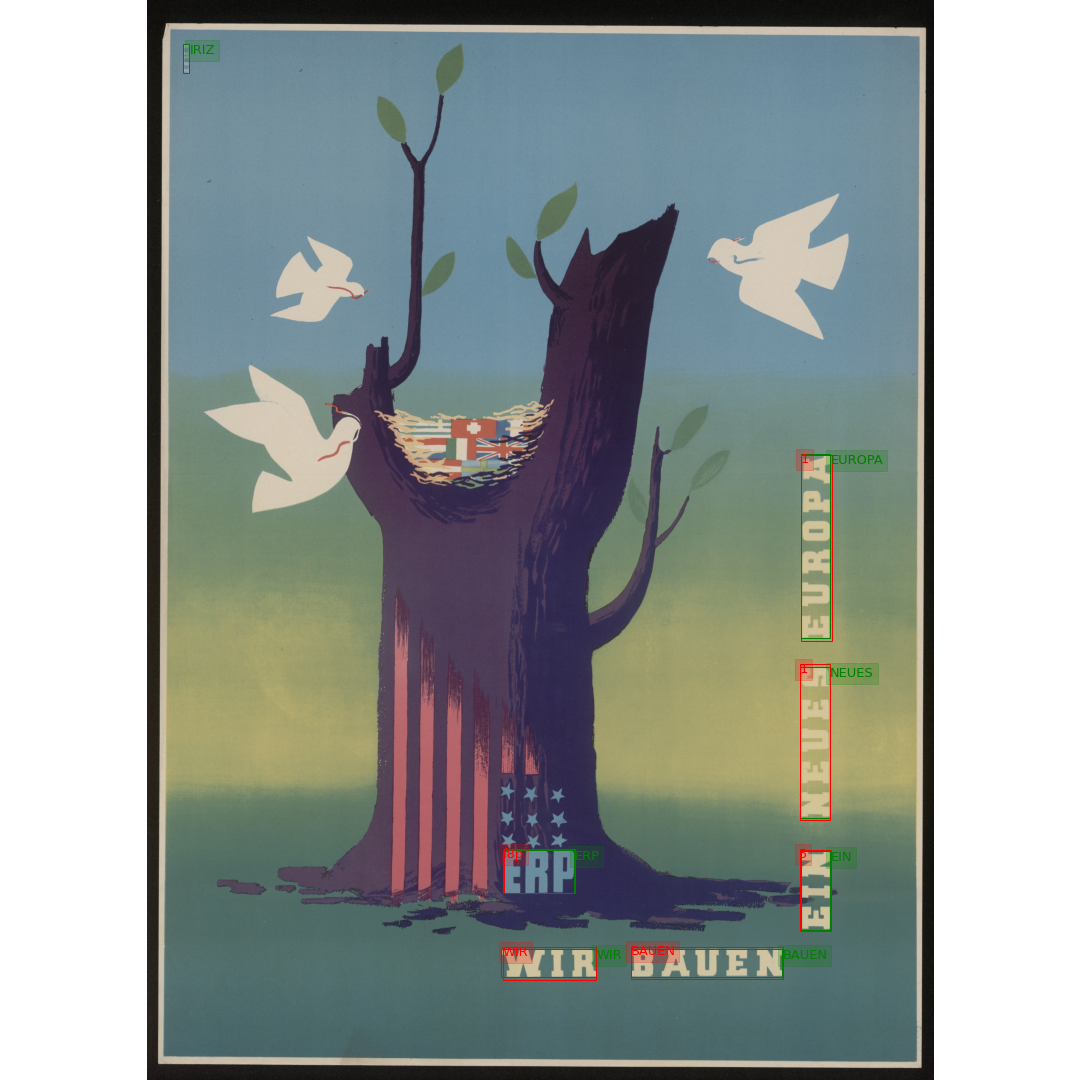
\includegraphics[width=\textwidth]{obrazky/plakaty/result_easyOCR_vienna1_split_tuning_special_sensitive-60verticaltextproblem.png}
    \caption{EasyOCR on image P-231248}
    \label{Im7:ex:easy}
\end{figure}


\subsection*{P-310877}
This image has a very specific font, which is, without former knowledge, very difficult to recognize.

\begin{figure}[hbtp!]
    \centering
    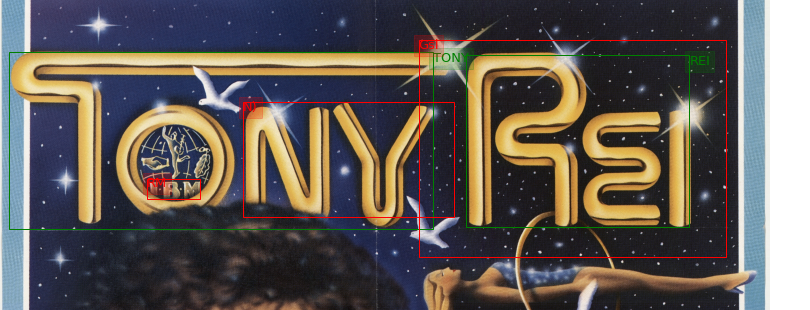
\includegraphics[width=\textwidth]{obrazky/plakaty/result_easyOCR_vienna2_nosplit_notuning_nocorrection-70.png}
    \caption{EasyOCR on image P-310877}
    \label{Im6:ex:easy}
\end{figure}




 % text vkládán ze souboru, kde je i příkaz \chapter{...}


\end{document} % SEM NESAHEJTE! Konec.
